\documentclass[10pt,a4paper]{article}
\usepackage[UTF8,fontset = windows]{ctex}
\setCJKmainfont[BoldFont=黑体,ItalicFont=楷体]{等线}
\usepackage{amssymb,amsmath,amsfonts,amsthm,mathrsfs,dsfont,graphicx}
\usepackage{ifthen,indentfirst,enumerate,color,titletoc}
\usepackage{tikz}
\usepackage{multicol}
\usepackage{makecell}
\usetikzlibrary{arrows,calc,intersections,patterns}
\usepackage[bf,small,indentafter,pagestyles]{titlesec}
\usepackage[top=1in, bottom=1in,left=0.8in,right=0.8in]{geometry}
\renewcommand{\baselinestretch}{1.65}
\newtheorem{defi}{定义~}
\newtheorem{eg}{例~}
\newtheorem{ex}{~}
\newtheorem{rem}{注~}
\newtheorem{thm}{定理~}
\newtheorem{coro}{推论~}
\newtheorem{axiom}{公理~}
\newtheorem{prop}{性质~}
\newcommand{\blank}[1]{\underline{\hbox to #1pt{}}}
\newcommand{\bracket}[1]{(\hbox to #1pt{})}
\newcommand{\onech}[4]{\par\begin{tabular}{p{.9\textwidth}}
A.~#1\\
B.~#2\\
C.~#3\\
D.~#4
\end{tabular}}
\newcommand{\twoch}[4]{\par\begin{tabular}{p{.46\textwidth}p{.46\textwidth}}
A.~#1& B.~#2\\
C.~#3& D.~#4
\end{tabular}}
\newcommand{\vartwoch}[4]{\par\begin{tabular}{p{.46\textwidth}p{.46\textwidth}}
(1)~#1& (2)~#2\\
(3)~#3& (4)~#4
\end{tabular}}
\newcommand{\fourch}[4]{\par\begin{tabular}{p{.23\textwidth}p{.23\textwidth}p{.23\textwidth}p{.23\textwidth}}
A.~#1 &B.~#2& C.~#3& D.~#4
\end{tabular}}
\newcommand{\varfourch}[4]{\par\begin{tabular}{p{.23\textwidth}p{.23\textwidth}p{.23\textwidth}p{.23\textwidth}}
(1)~#1 &(2)~#2& (3)~#3& (4)~#4
\end{tabular}}
\begin{document}
\begin{enumerate}[1.]

\item 若全集$U=\{x|x^2-7x+12\le 0\}$, 集合$M=\{x|3<x<4\}$, $N=\left\{x\left|\dfrac{x-3}{4-x}\ge 0\right.\right\}$, 则$\complement_U M\cap \complement_U N=$\blank{50}.
\item 设$\alpha:2\le x\le 4$, $\beta: m+1\le x\le 2m+4, \ m\in \mathbf{R}$, 如果$\alpha$是$\beta$的充分非必要条件, 则$m$的范围是\blank{50}.
\item 若函数$y=a^x+b$($a>0$且$a\ne 1$)的图像经过点$(1,7)$, 其反函数的图像经过点$(4,0)$, 则$a-b=$\blank{50}.
\item 已知$\sin\theta=\dfrac 14$, 则$\sin\left[2\left(\theta-\dfrac\pi 4\right)\right]=$\blank{50}.
\item 已知圆锥的母线长为$a$, 轴截面(过轴的截面)为直角三角形, 则圆锥的全面积为\blank{50}.
\item 函数$f(x)=2+\sin x-\tan 2x$, 如果$f(a)=1$, 则$f(-a)=$\blank{50}.
\item 设$S_n$是等差数列$\{a_n\}$的前$n$项和. 若$\dfrac{S_3}{S_7}=\dfrac 13$, 则$\dfrac{S_6}{S_7}=$\blank{50}.
\item 若关于$x$的不等式$|x-3|-|x+2|>a$恒成立, 则实数$a$的范围是\blank{50}.
\item 若$S_n=\dfrac 15+\dfrac {2}{5^2}+\dfrac {1}{5^3}+\dfrac{2}{5^4}+\cdots+\dfrac{1}{5^{2n-1}}+\dfrac{2}{5^{2n}}$, 则$\displaystyle\lim_{n\to \infty}S_n=$\blank{50}.
\item 若函数$f(x)=ax^2+bx+c\ (a>0)$, 不等式$ax^2+bx+c<0$的解集为$\{x|-2<x<0\}$, 当$0<n<m$时, $f(n),f(m),f(\sqrt{mn}),f\left(\dfrac{m+n}2\right)$这四个值中最大的一个是\blank{50}.
\item 设地球半径为$R$, 甲地位于北纬$45^\circ$东经$105^\circ$, 乙地位于南纬$30^\circ$东经$105^\circ$, 则甲乙两地间的球面距离是\blank{30}.
\fourch{$\dfrac{5\pi}{12}R$}{$\dfrac{7\pi}{12}R$}{$\dfrac{\sqrt{2}}2R$}{$\dfrac{\sqrt{3}}2R$}
\item 已知函数$f(x)=\begin{cases}
\log_2(x+4), & x\ge 0,\\f(x+1)-f(x+2), & x<0,\end{cases}$ 则$f(-3)$的值为\blank{30}.
\fourch{$1$}{$0$}{$2$}{$-2$}
\item 若集合$A=\{x|x^2-2x<0\}$, $B=\{x||x|<1\}$, 则$A\cup B$等于\blank{50}.
\item 函数$y=\sqrt{2016^{1-x}}$的定义域是\blank{50}.
\item 已知函数$f(x)=\begin{vmatrix}
1&1\\1&\log_2 x
\end{vmatrix}$, 则$f^{-1}(1)=$\blank{50}.
\item 若复数$\dfrac{1+\mathrm{i}}{1-\mathrm{i}}+\dfrac 12 b \ (b\in \mathbf{R})$的实部的绝对值与虚部相等, 则$b$的值为\blank{50}.
\item 已知$p$为常数, $a_n=\begin{cases}
\dfrac{2n-1}{n+1}, &1\le n\le 2016,\\\left(1+\dfrac 1n\right)^p, & n>2016,
\end{cases}$ 则$\displaystyle\lim_{n\to \infty}a_n=$\blank{50}.
\item 若一个圆锥的母线与轴的夹角为$\arcsin\dfrac 13$, 则该圆锥的侧面积是底面积的\blank{50}倍.
\item 设$x\in\mathbf{R}$, 向量$\overrightarrow{a}=(x,1)$, $\overrightarrow{b}=(1,2)$, 且$\overrightarrow{a}\perp \overrightarrow{b}$, 则$|\overrightarrow{a}+\overrightarrow{b}|=$\blank{50}.
\item 若函数$f(x)=\dfrac{k-2^x}{1+k\cdot 2^x}, \ (k\ne 1, \ k\in \mathbf{R})$在定义域内为奇函数, 则$k=$\blank{50}.
\item 从集合$\{0,1,2,3\}$的所有非空子集中, 等可能地取出一个. 则取出的非空子集中所有元素之和恰为$5$的概率为\blank{50}.
\item (理科)若对于任意的实数$x\in \mathbf{R}$, 不等式$2x^2-a\sqrt{1+x^2}+3\ge 0$恒成立, 则实数$a$的取值范围为\blank{50}.
\item ``$(2x+1)x=0$''是``$x=0$''的\blank{30}.
\twoch{充分不必要条件}{必要不充分条件}{充分必要条件}{既不充分也不必要条件}
\item 下列函数中, 与函数$y=x^{2n+1} \ (n\in \mathbf{N}^*)$的值域相同的函数为\blank{30}.
\fourch{$y=\left(\dfrac 12\right)^{x+1}$}{$y=\ln(x+1)$}{$y=\dfrac{x+1}{x}$}{$y=x+\dfrac 1x$}
\item 函数$f(x)=x\cos 2x$在区间$[0,2\pi]$上的零点的个数为\blank{30}.
\fourch{$2$}{$3$}{$4$}{$5$}
\item 函数$f(x)=\sqrt{27-3^{2x+1}}$的定义域是\blank{50}.(用区间表示)
\item 已知椭圆中心在原点, 一个焦点为$F(-2\sqrt{3},0)$, 且长轴长是短轴长的$2$倍, 则该椭圆的标准方程是\blank{50}.
\item 实践中常采用``捉--放--捉''的方法估计一个鱼塘中鱼的数量. 如从这个鱼塘中随机捕捞出$100$条鱼, 将这$100$条鱼分别作一记号后再放回鱼塘, 数天后再从鱼塘中随机捕捞出$108$条鱼, 其中有记号的鱼有$9$条, 从而可以估计出鱼塘中的鱼约有\blank{50}条.
\item 若二项式$\left(ax-\dfrac{\sqrt{3}}{6}\right)^3$的展开式的第二项系数为$-\dfrac{\sqrt{3}}{2}$, 则实数$a$的值为\blank{50}.
\item 在$\triangle ABC$中, 角$A,B,C$的对边分别为$a,b,c$. 若$b=\sqrt{5}$, $\angle B=\dfrac{\pi}{4}$, $\tan A=2$, 则$a$等于\blank{50}.
\item 已知数列$\{a_n\}$满足$a_1=a_2=1$, $\dfrac{a_{n+2}}{a_{n+1}}-\dfrac{a_{n+1}}{a_n}=1$, 则$a_6-a_5$的值为\blank{50}.
\item 直线$x=0$, $y=0$与曲线$y=\sqrt{4-x^2}$所围成的图形绕$x$轴旋转一周而成的旋转体的体积等于\blank{50}.
\item 点$P$在双曲线$\dfrac{x^2}{a^2}-\dfrac{y^2}{b^2}=1 \ (a>0, \ b>0)$上, $F_1,F_2$是该双曲线的两个焦点, $\angle F_1PF_2=90^\circ$, 且$\triangle F_1PF_2$的三条边长成等差数列, 则$a:b=$\blank{50}.
\item (理科)直角坐标系$xOy$中, 以原点为极点, $x$轴的正半轴为极轴建立极坐标系, 已知曲线$C_1: \begin{cases}x=2+2\cos\theta, \\y=2\sin \theta,\end{cases}$($\theta$为参数) 曲线$C_2:\rho\cos\left(\theta+\dfrac{\pi}{3}\right)=t$, 若两曲线有公共点, 则实数$t$的取值范围是\blank{50}.
\item 已知$a>b$, 二次三项式$ax^2+2x+b\ge 0$对于一切实数$x$恒成立. 又存在$x_0\in \mathbf{R}$, 使得$ax_0^2+2x_0+b=0$成立, 则$\dfrac{a^2+b^2}{a-b}$的最小值为\blank{50}.
\item 若$a,b,c\in \mathbf{R}$, 且$a>b$, 则下列不等式一定成立的是\blank{30}.
\fourch{$a+c\ge b-c$}{$ac>bc$}{$\dfrac{c^2}{a-b}>0$}{$(a-b)c^2\ge 0$}
\item 设数列$\{a_n\}$, 下列正确的是\blank{30}.
\onech{若$a_n^2=4^n, \ n\in \mathbf{N}$, 则$\{a_n\}$为等比数列}
{若$a_n\cdot a_{n+2}=a_{n+1}^2, \ n\in\mathbf{N}^*$, 则$\{a_n\}$为等比数列}
{若$a_m\cdot a_n=2^{m+n}, \ m,n\in \mathbf{N}$, 则$\{a_n\}$为等比数列}
{若$a_n\cdot a_{n+3}=a_{n+1}\cdot a_{n+2}, \ n\in \mathbf{N}$, 则$\{a_n\}$为等比数列}
\item 我们规定``渐近线''的概念: 已知曲线$C$, 如果存在有一条直线, 当曲线$C$上任一点$M$沿曲线运动时$M$可无限趋近于该直线但永远达不到, 那么这条直线称为这条曲线的``渐近线''. 下列函数

\textcircled{1} $f(x)=x^2+2x-3$, \textcircled{2} $g(x)=2^x+1$, \textcircled{3} $h(x)=\log_2(x-1)$, \textcircled{4} $t(x)=\dfrac{2x+1}{x-1}$, \textcircled{5} $u(x)=\dfrac{x^2+2}{x}$, 其中有``渐近线''的个数为\blank{30}.
\fourch{$2$}{$3$}{$4$}{$5$}
\item 已知集合$A=\{y|y=\sin x, \ x\in \mathbf{R}\}$, $B=\{x|x(2-x)>0\}$, 则$A\cup B=$\blank{50}.
\item 幂函数$f(x)$的图像经过点$(2,\sqrt{2})$, 且$f^{-1}(x)$为$f(x)$的反函数, 则$f^{-1}(4)=$\blank{50}.
\item 若$\log_a \dfrac 23<1 \ (a>0, \ a\ne 1)$, 则实数$a$的取值范围为\blank{50}.
\item (理科)设曲线$C$定义为到点$(-1,-1)$和$(1,1)$距离之和为$4$的动点的轨迹. 若将曲线$C$绕坐标原点逆时针旋转$45^\circ$, 则此时曲线$C$的方程为\blank{50}.\\
(文科)椭圆$2x^2+3y^2=6$的焦距为\blank{50}.
\item 已知无穷等比数列$\{a_n\}$的各项和为$4$, 则首项$a_1$的取值范围为\blank{50}.
\item 已知$\left(\sqrt{x}+\dfrac 3{\sqrt[3]{x}}\right)^n$展开式中, 各项系数的和与各项二项式系数的和之差为$56$, 则$n=$\blank{50}.
\item (理科)设口袋中有黑球、白球共$7$个, 从中任取$2$个球, 已知取到的白球的个数的数学期望为$\dfrac 6 7$, 则口袋中白球的个数为\blank{50}.\\
(文科)从$0,1,2,3,4$这五个数中随机取$2$个数组成一个二位数, 则这个二位数为偶数的概率是\blank{50}.
\item 一个正三棱锥的四个顶点都在半径为$1$的球面上, 其中底面的三个顶点在该球的一个大圆上, 则该正三棱锥的体积是\blank{50}.
\item 将边长为$1$米的正三角形薄片, 沿一条平行于底边的直线剪成两块, 其中一块是梯形, 记$S=\dfrac{(\text{梯形的周长})^2}{\text{梯形的面积}}$, 则$S$的最小值是\blank{50}.
\item 定义区间$(c,d),(c,d],[c,d),[c,d]$的长度均为$d-c\ (d>c)$. 若$a\ne 0$, 关于$x$的不等式$x^2-\left(2a+\dfrac 1a\right)x-1<0$的非空解集(用区间表示)记为$I(a)$, 则当区间$I(a)$的长度取得最小值时, 实数$a$的值为\blank{50}.
\item 过点$(1,0)$且与直线$x-2y-2=0$的法向量垂直的直线方程是\blank{30}.
\twoch{$x-2y+1=0$}{$2x+y-2=0$}{$x+2y-1=0$}{$x-2y-1=0$}
\item (理科)在极坐标中, 与点$\left(2,\dfrac{\pi}{3}\right)$关于极点对称的点的一个极坐标是\blank{30}.
\fourch{$\left(-2,-\dfrac{\pi}{3}\right)$}{$\left(2,-\dfrac{\pi}{3}\right)$}{$\left(2,-\dfrac{2\pi}{3}\right)$}{$\left(-2,\dfrac{4\pi}{3}\right)$}\\
(文科)如果实数$x,y$满足条件$\begin{cases}
x-y+1\ge 0,\\y+1\ge 0,\\x+y+1\le 0,
\end{cases}$ 那么$2x-y$的最大值为\blank{30}.
\fourch{$2$}{$1$}{$-2$}{$-3$}
\item 设函数$f(x)=x^3+\dfrac{2^x-1}{2^x+1}$, 已知$a\in (-1,1)$, $b\in (-1,1)$. 则$a+b\ge 0$是$f(a)+f(b)\ge 0$的\blank{30}.
\twoch{充分不必要条件}{必要不充分条件}{充分必要条件}{既不充分也不必要条件}
\item 已知$a\in\mathbf{R}$, 命题$P:$``实系数一元二次方程$x^2+ax+2=0$的两根都是虚数''; 命题$Q:$``存在复数$z$同时满足$|z|=2$且$|z+a|=1$''.

是判断命题$P$和命题$Q$之间是否存在推出关系? 说明你的理由.
\item 已知公差不为$0$的等差数列$\{a_n\}$的首项$a_1$为$a \ (a\in \mathbf{R})$, 设数列的前$n$项和为$S_n$, 且$\dfrac{1}{a_1},\dfrac{1}{a_2},\dfrac{1}{a_4}$成等比数列.\\
(1) 求数列$\{a_n\}$的通项公式及$S_n$;\\
(2) 记$A_n=\dfrac{1}{S_1}+\dfrac{1}{S_2}+\dfrac{1}{S_3}+\cdots+\dfrac{1}{S_n}$, $B_n=\dfrac{1}{a_1}+\dfrac{1}{a_2}+\dfrac{1}{a_{2^2}}+\cdots+\dfrac{1}{a_{2^{n-1}}}$, 当$n\ge 2$时, 试比较$A_n$和$B_n$的大小.
\item 已知集合$A=\{1,3,\sqrt{m}\}$, $B=\{1,m\}$, $A\cup B=A$, 则$m=$\blank{50}.
\item 若$\begin{vmatrix}
x^2 & y^2\\-1 & 1
\end{vmatrix}=\begin{vmatrix}
x & x \\ y & -y
\end{vmatrix}$, 则$x+y=$\blank{50}.
\item 若$\dfrac{3+b\mathrm{i}}{a+b\mathrm{i}}=1-\mathrm{i}$($a,b$为实数, $\mathrm{i}$为虚数单位), 则$a+b=$\blank{50}.
\item 已知递增的等差数列$\{a_n\}$满足$a_1=1$, $a_3=a_2^2-4$, 则$a_n=$\blank{50}.
\item 设常数$a\in \mathbf{R}$, 若$\left(x^2+\dfrac ax\right)^5$的二项展开式中$x^7$的系数为$-10$, 则$a=$\blank{50}.
\item 已知双曲线$C_1: \dfrac{x^2}{a^2}-\dfrac{y^2}{b^2}=1 \ (a>0,\ b>0)$与双曲线$C_2: \dfrac{x^2}{4}-\dfrac{y^2}{16}=1$有相同的渐近线, 且$C_1$的右焦点为$F(\sqrt{5},0)$, 则$a=$\blank{50}, $b=$\blank{50}.
\item (理科)如图, 在极坐标系中, 过点$M(2,0)$的直线$l$与极轴的夹角$\alpha=\dfrac{\pi}{6}$, 若将$l$的极坐标方程写成$\rho=f(\theta)$的形式, 则$f(\theta)=$\blank{50}.
\begin{center}
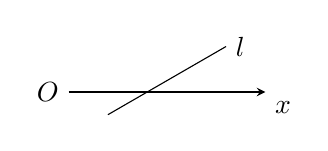
\begin{tikzpicture}[>=stealth]
\draw [->](0,0) node [left] {$O$}--(2.5,0) node [below right]{$x$};
\draw (0.5,{-0.5/sqrt(3)})--(2,{1/sqrt(3)}) node [right] {$l$};
\end{tikzpicture}
\end{center}



\item 某学校组织学生参加英语测试, 成绩的频率分布直方图如图, 数据的分组依次为$[20,40),[40,60),[60,80),[80,100)$. 若低于$60$分的人数是$15$人, 则该班的学生人数是\blank{50}.
\begin{center}
	\begin{tikzpicture}[>=stealth]
	\draw [->](-0.5,0)--(0,0) node [below left] {$O$}--(3,0) node [below right]{成绩$/$分};
	\draw [->] (0,-0.5)--(0,2) node [left] {$\dfrac{\text{频率}}{\text{组距}}$};
	\draw (0.5,0)--(0.5,0.3)--(1,0.3) (1,0)--(1,0.6)--(1.5,0.6) (1.5,0)--(1.5,1.2)--(2,1.2)--(2,0) (2,0.9)--(2.5,0.9)--(2.5,0);
	\draw (0,0.3) node [left] {$0.005$};
	\draw (0,0.6) node [left] {$0.01$};
	\draw (0,0.9) node [left] {$0.015$};
	\draw (0,1.2) node [left] {$0.02$};
	\draw (0.5,0) node [below] {$20$};
	\draw (1,0) node [below] {$40$};
	\draw (1.5,0) node [below] {$60$};
	\draw (2,0) node [below] {$80$};
	\draw (2.5,0) node [below] {$100$};
	\draw [dashed] (0,0.3)--(0.5,0.3) (0,0.6)--(1,0.6) (0,0.9)--(2,0.9) (0,1.2)--(1.5,1.2);
	\end{tikzpicture}
\end{center}



\item (理科)已知正四棱柱$ABCD-A_1B_1C_1D_1$中, $AA_1=2AB$, 则$CD$与平面$BDC_1$所成角的正弦值等于\blank{50}.
\item $f(x)$是定义在$\mathbf{R}$上且周期为$2$的函数, 在区间$[-1,1]$上, $f(x)=\begin{cases}ax+1, & -1\le x<0,\\\dfrac{bx+2}{x+1}, & 0\le x\le 1,\end{cases}$ 其中$a,b\in \mathbf{R}$. 若$f\left(\dfrac 12\right)=f\left(\dfrac 32\right)$, 则$a+3b$的值为\blank{50}.
\item 函数$f(x)=2^x+x^3-2$在区间$(0,1)$内的零点的个数是\blank{30}.
\fourch{$0$}{$1$}{$2$}{$3$}
\item 设$\overrightarrow{a},\overrightarrow{b}$都是非零向量, 下列四个条件中, 使$\dfrac{\overrightarrow{a}}{|\overrightarrow{a}|}=\dfrac{\overrightarrow{b}}{|\overrightarrow{b}|}$成立的充分条件是\blank{30}.
\twoch{$|\overrightarrow{a}|=|\overrightarrow{b}|$且$\overrightarrow{a}\parallel \overrightarrow{b}$}{$\overrightarrow{a}=-\overrightarrow{b}$}{$\overrightarrow{a}\parallel\overrightarrow{b}$}{$\overrightarrow{a}=2\overrightarrow{b}$}
\item 定义在$(-\infty,0)\cup (0,+\infty)$上的函数$f(x)$, 如果对于任意给定的等比数列$\{a_n\}$, $\{f(a_n)\}$仍是等比数列, 则称$f(x)$为``保等比数列函数''. 现有定义在$(-\infty,0)\cup (0,+\infty)$上的如下函数: \textcircled{1} $f(x)=x^2$; \textcircled{2} $f(x)=2^x$; \textcircled{3} $f(x)=\sqrt{|x|}$; \textcircled{4} $f(x)=\ln|x|$. 则其中是``保等比数列函数''的$f(x)$的序号为\blank{30}.
\fourch{\textcircled{1}\textcircled{2}}{\textcircled{3}\textcircled{4}}{\textcircled{1}\textcircled{3}}{\textcircled{2}\textcircled{4}}
\item 在锐角$\triangle ABC$中, $a,b,c$分别为内角$A,B,C$所对的边, 且满足$\sqrt{3}a-2b\sin A=0$.\\
(1) 求角$B$的大小;\\
(2) 若$a+c=5$, 且$a>c$, $b=\sqrt{7}$, 求$\triangle ABC$的面积.
\item 已知集合$A=\left\{x\left|\dfrac{2x+1}{x+2}<1, \ x\in \mathbf{R}\right.\right\}$, 函数$f(x)=|mx+1| \ (m\in \mathbf{R})$. 函数$g(x)=x^2+ax+b \ (a,b\in \mathbf{R})$的值域为$[0,+\infty)$.\\
(1) 若不等式$f(x)<3$的解集为$A$, 求$m$的值;\\
(2) 在(1)的条件下, 若$\left|f(x)-2f\left(\dfrac x 2\right)\right|\le k$恒成立, 求$k$的取值范围;\\
(3) 若关于$x$的不等式$g(x)<c$的解集为$(m,m+6)$, 求实数$c$的值.
\item 已知$U=\left\{y\left|y=\log_\frac 12 x, \ x\ge \dfrac 18\right.\right\}$, $A=\left\{x\left|y=\dfrac{1}{\sqrt{2-x}}\right.\right\}$, 则$\complement_U A=$\blank{50}.
\item 命题``已知$x,y\in \mathbf{R}$,  若$x+y>2$, 则$x>1$且$y>1$''的否命题是\blank{150}; 该否命题是\blank{50}命题(填``真'',``假'').
\item 若存在实数$a$, 使得关于$x$的不等式$ax+b>x+1$的解集为$\{x|x<1\}$, 则实数$b$的取值范围为\blank{50}.
\item 已知函数$f(x)=4^x-k\cdot 2^{x+1}+4$在$[0,2]$上存在零点, 则实数$k\in$\blank{50}.
\item 若在$\triangle ABC$中, $2\sin^2A-3\cos A=0$, 则角$A$的大小为\blank{50}.
\item (理科)在极坐标系中, 若过点$(3,0)$且与极轴垂直的直线交曲线$\rho=4\cos\theta$于$A,B$两点, 则$|AB|=$\blank{50}.
\item 已知直线$l_1:4x-3y+6=0$和直线$l_2:x+1=0$, 抛物线$y^2=4x$上的动点$P$到直线$l_1$和$l_2$的距离之和的最小值为\blank{50}.
\item 若等比数列$\{a_n\}$中$a_2=1$, 则其前$3$项的和$S_3$的取值范围为\blank{50}.
\item (理科)已知$f(x)$是$\mathbf{R}$上的奇函数, $g(x)$是$\mathbf{R}$上的偶函数, 若函数$f(x)+g(x)$的值域为$[1,3)$, 则$f(x)-g(x)$的值域为\blank{50}.\\
(文科)已知$f(x)$是$\mathbf{R}$上的奇函数, $g(x)$是$\mathbf{R}$上的偶函数, 若函数$f(x)+g(x)$的值域为$[1,3)$, 则$f(-x)+g(x)$的值域为\blank{50}.
\item 给定两个长度为$1$的平面向量$\overrightarrow{OA}$和$\overrightarrow{OB}$, 它们的夹角为$120^\circ$. 如图所示, 点$C$在以$O$为圆心的圆弧$AB$上变动. 若$\overrightarrow{OC}=x\overrightarrow{OA}+y\overrightarrow{OB}$, 其中$x,y\in \mathbf{R}$, 则$x+y$的最大值是\blank{50}.
\begin{center}
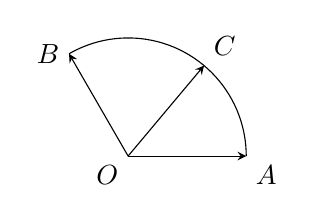
\begin{tikzpicture}[>=stealth]
\draw [->] (0,0) node [below left] {$O$}--(1.5,0) node [below right] {$A$};
\draw [->] (0,0)--({-1.5/2},{0.75*sqrt(3)}) node [left]{$B$};
\draw (1.5,0) arc (0:120:1.5);
\draw [->] (0,0)--({1.5*cos(50)},{1.5*sin(50)}) node [above right] {$C$};
\end{tikzpicture}
\end{center}
\item 已知函数$f(x)=2\sin\left(\dfrac x2+\dfrac \pi 3\right)$, 若对任意的$x\in \mathbf{R}$都有$f(x_1)\le f(x)\le f(x_2)$, 则$|x_1-x_2|$的最小值为\blank{30}.
\fourch{$\dfrac \pi 3$}{$\dfrac{2\pi}{3}$}{$2\pi$}{$4\pi$}
\item 若数列$\{b_n\}$为等比数列, 其前$n$项的和为$S_n$, 若对任意$n\in \mathbf{N}^*$, 点$(n,S_n)$均在函数$y=bx+r$($b>0, \ b\ne 1, \ b,r$为常数)的图像上, 则$r=$\blank{30}.
\fourch{$0$}{$-1$}{$1$}{$2$}
\item ``顺数''是指在一个整数中, 每一位数字比其左边的一位数字大(除首位数字外), 如$24567$就是一个五位``顺数''. 任取一个两位``顺数'', 该数大于$56$的概率为\blank{30}.
\fourch{$\dfrac 13$}{$\dfrac 14$}{$\dfrac {7}{12}$}{$\dfrac{5}{16}$}
\item 如图: 直三棱柱$ABC-A'B'C'$内接于高为$\sqrt{2}$的圆柱中, 已知$\angle ACB=90^\circ$, $AA'=\sqrt{2}$, $BC=AC=1$, $O$为$AB$的中点. \\
(1) 求圆柱的全面积;\\
(2) (文科)求异面直线$AB'$与$CO$所成的角的大小.\\
(理科)求二面角$A'-BC-A$的大小.
\begin{center}
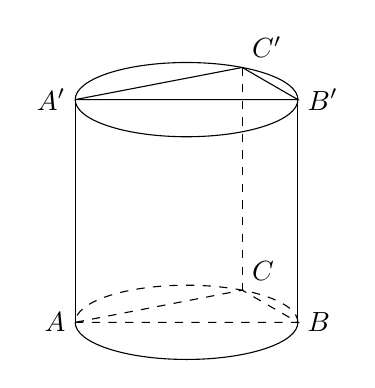
\begin{tikzpicture}
\draw [dashed] (0,0) arc (0:180:{sqrt(2)} and {sqrt(2)/3});
\draw (0,0) arc (0:-180:{sqrt(2)} and {sqrt(2)/3});
\draw (0,{2*sqrt(2)}) arc (0:180:{sqrt(2)} and {sqrt(2)/3});
\draw (0,{2*sqrt(2)}) arc (0:-180:{sqrt(2)} and {sqrt(2)/3});
\draw (0,0)--(0,{2*sqrt(2)}) ({-2*sqrt(2)},0)--({-2*sqrt(2)},{2*sqrt(2)});
\draw [dashed] ({-2*sqrt(2)},0)node [left] {$A$}--(0,0) node [right] {$B$}--({-sqrt(2)+sqrt(2)*cos(60)},{sqrt(2)/3*sin(60)}) node [above right] {$C$}--cycle;
\draw  ({-2*sqrt(2)},{2*sqrt(2)}) node [left] {$A'$}--(0,{2*sqrt(2)}) node [right] {$B'$}--({-sqrt(2)+sqrt(2)*cos(60)},{sqrt(2)/3*sin(60)+2*sqrt(2)}) node [above right] {$C'$}--cycle;
\draw [dashed] ({-sqrt(2)+sqrt(2)*cos(60)},{sqrt(2)/3*sin(60)+2*sqrt(2)})--({-sqrt(2)+sqrt(2)*cos(60)},{sqrt(2)/3*sin(60)});
\end{tikzpicture}
\end{center}
\item 设函数$f(x)=\log_\frac 12 x$, $g(x)=f^{-1}(|x|)$.\\
(1) 求函数$g(x)$的解析式, 并画出大致图像;\\
(2) 若不等式$g(x)+g(2x)\le k$对任意$x\in \mathbf{R}$恒成立, 求实数$k$的取值范围.
\item 已知$f(x)=1-x^2 \ (x<-1)$, 则$f^{-1}(-3)=$\blank{50}.
\item 已知$\alpha\in \left(\dfrac{\pi}{2},\pi\right)$, $\sin\alpha=\dfrac{3}{5}$, 则$\tan\left(\alpha+\dfrac{\pi}{4}\right)=$\blank{50}.
\item 若关于$x,y$的二元线性方程组的增广矩阵为$\begin{pmatrix}1 & 3 & 5\\2 & 4 & 6\end{pmatrix}$, 则$x-y=$\blank{50}.
\item 已知某圆锥的体积是$12\pi$cm$^2$, 底面半径等于$3$cm, 则该圆锥的高为\blank{50}.
\item 若复数$z=\left(\dfrac 12-\dfrac{\sqrt{3}}{2}\mathrm{i}\right)^2$是实系数方程$ax^2+bx+1=0$的根, 则$a\cdot b=$\blank{50}.
\item 某抛物线形拱桥的跨度为$20$米, 拱高是$4$米, 在建桥时, 每隔$4$米需用一根支柱支撑, 其中最高支柱的高度是\blank{50}米.(答案保留两位小数)
\item (理科)化极坐标方程$(\rho-2)\left(\theta-\dfrac{\pi}{3}\right)=0$为直角坐标方程: \blank{100}.
\item 设$x,y$均为正实数, 且$\dfrac{1}{2+x}+\dfrac{1}{2+y}=\dfrac 14$, 则$xy$的最小值为\blank{50}.
\item 三角形的三内角$A,B,C$所对边的长分别为$a,b,c$, 设向量$\overrightarrow{m}=(a-b,a-c)$, $\overrightarrow{n}=(c,a+b)$. 若$\overrightarrow{m}\parallel \overrightarrow{n}$, 则角$B$的大小为\blank{50}.
\item 已知$f(x)=4-\dfrac 1x$, 若存在区间$[a,b]\subseteq \left(\dfrac 13,+\infty\right)$, 使得$\{y|y=f(x), \ x\in [a,b]\}=[ma,mb]$, 则实数$m$的取值范围是\blank{50}.
\item 下列命题中正确的是\blank{30}.
\twoch{若$ac>bc$, 则$a>b$}{若$a^2>b^2$, 则$a>b$}{若$\dfrac 1a>\dfrac 1b$, 则$a<b$}{若$\sqrt{a}<\sqrt{b}$, 则$a<b$}
\item 下列函数中, 既是偶函数, 又是在区间$(0,+\infty)$上单调递减的函数为\blank{30}.
\fourch{$y=\lg\dfrac{1}{|x|}$}{$y=x^3$}{$y=3^{|x|}$}{$y=x^2$}
\item 已知数列$\{a_n\}$是等差数列, 则``$a_1+a_9<a_4+a_7$''是``$\{a_n\}$为递增数列''的\blank{30}.
\twoch{充分非必要条件}{必要非充分条件}{充要条件}{既非充分又非必要条件}
\item 某校高一年级开设研究性学习课程, 一班和二班报名参加的人数分别是$18$和$27$. 现用分层抽样的方法, 从中抽取若干名学生组成研究性学习小组, 已知从二班抽取了$3$名同学.\\
(1) 求研究性学习小组的人数;\\
(2) 规划在研究性学习的中、后期各安排$1$次交流活动, 每次随机抽取小组中$1$名同学发言. 求$2$次发言的学生恰好来自不同班级的概率.
\item 已知点$A(-1,0)$, $B(1,0)$, $C\left(-\dfrac{5\sqrt{7}}{12},0\right)$, $D\left(\dfrac{5\sqrt{7}}{12},0\right)$, 动点$P(x,y)$满足$\overrightarrow{AP}\cdot\overrightarrow{BP}=0$, 动点$Q(x,y)$满足$|\overrightarrow{QC}|+|\overrightarrow{QD}|=\dfrac{10}{3}$.\\
(1) 求动点$P$的轨迹方程$C_0$和动点$Q$的轨迹方程$C_1$;\\
(2) 是否存在与曲线$C_0$外切且与曲线$C_1$内接的平行四边形? 若存在, 请求出{\bf 一个}这样的四边形; 若不存在, 说明理由;\\
(3) 固定曲线$C_0$, 在(2)的基础上提出一个一般性的问题, 使(2)成为(3)的特例, 探究能得出相应结论(或加强结论)需满足的条件, 并说明理由.
\item 已知命题$p:$``若$\overrightarrow{a}=\overrightarrow{b}$, 则$|\overrightarrow{a}|=|\overrightarrow{b}|$'', 则命题$p$及其逆命题, 否命题, 逆否命题中, 正确命题的个数是\blank{50}.
\item 在一次教师联欢会上, 到会的女教师比男教师多$12$人, 从到会教师中随机挑选一人表演节目. 如果每位教师被选中的概率相等, 而且选中男教师的概率为$\dfrac 9{20}$, 那么参加这次联欢会的教师共有\blank{50}人.
\item 在$\triangle ABC$中, $C=60^\circ$, $AB=\sqrt{3}$, $BC=\sqrt{2}$, 那么$A=$\blank{50}.
\item 设$A,B,C$是圆$x^2+y^2=1$上不同的三个点, $O$为圆心, 且$\overrightarrow{OA}\cdot\overrightarrow{OB}=0$, 存在实数$\lambda,\mu$使得$\overrightarrow{OC}=\lambda\overrightarrow{OA}+\mu\overrightarrow{OB}$, 则实数$\lambda$和$\mu$的关系为\blank{50}.
\item 如下图所示的程序框图中, 循环体执行的次数是\blank{50}.
\begin{center}
\begin{tikzpicture}[>=stealth]
\draw (0,-0.3)--(1,-0.3) arc (-90:90:0.3)--(0,0.3) arc (90:270:0.3);
\draw (0.5,0) node {开始};
\draw [->] (1.3,0)--(1.6,0);
\draw (1.6,-0.3) rectangle (4,0.3);
\draw (2.8,0) node {$i=2, \ S=0$};
\draw [->] (4,0)--(4.3,0);
\draw (4.3,-0.3) rectangle (6.3,0.3);
\draw (5.3,0) node {$S=S+i$};
\draw [->] (6.3,0)--(6.6,0);
\draw (6.6,-0.3) rectangle (8.6,0.3);
\draw (7.6,0) node {$i=i+2$};
\draw [->] (8.6,0)--(8.9,0);
\draw [->] (8.9,0)--(10,0.5)--(11.1,0)--(10,-0.5)--cycle;
\draw (10,0) node {$i\ge 100$};
\draw [->] (11.1,0) node [above right] {是}--(12,0);
\draw (11.7,-0.3)--(12.3,0.3)--(14.1,0.3)--(13.5,-0.3)--cycle;
\draw (12.9,0) node {输出$S$};
\draw [->] (13.8,0)--(14.1,0);
\draw (14.4,-0.3)--(15.4,-0.3) arc (-90:90:0.3)--(14.4,0.3) arc (90:270:0.3);
\draw (14.9,0) node {结束};
\draw [->] (10,-0.5) node [below right] {否}--(10,-1)--(4.15,-1)--(4.15,0);
\end{tikzpicture}
\end{center}


\item 设常数$a>0$, 若对任意正实数$x,y$, 不等式$(x+y)\cdot\left(\dfrac 1x+\dfrac ay\right)\ge 9$恒成立, 则$a$的最小值为\blank{50}.
\item 若$(1-2x)^{2014}=a_0+a_1x+a_2x^2+\cdots+a_{2014}x^{2014} \ (x\in \mathbf{R})$, 则$\dfrac{a_1}{2}+\dfrac{a_2}{2^2}+\cdots+\dfrac{a_{2014}}{2^{2014}}$的值为\blank{50}.
\item 若三个人踢毽, 互相传递, 每人每次只能踢以下, 由甲开始踢, 经过$5$次传递后, 毽又被踢回给甲, 则不同的传递方式共有\blank{50}种.
\item 在数列$\{a_n\}$中, 若$a_n^2-a_{n+1}^2=p\ (n\ge 1, \ n\in\mathbf{N}^*, \ p$为常数$)$, 则称$\{a_n\}$为``等方差数列''. 下列是对``等方差数列''的判断,

\textcircled{1} 若$\{a_n\}$是等方差数列, 则$\{a_n^2\}$是等差数列;

\textcircled{2} $\{(-1)^n\}$是等方差数列;

\textcircled{3} 若$\{a_n\}$是等方差数列, 则$\{a_{kn}\} \ (k\in \mathbf{N}^*, \ k$为常数$)$也是等方差数列.

其中真命题的序号为\blank{50}(将所有真命题的序号填写在横线上).
\item (理科)在极坐标系中, 圆$\rho=2\cos\theta$的圆心到直线$\rho\cos\theta=2$的距离是\blank{50}.
\item 在同一坐标系中画出函数$y=\log_a x, \ y=a^x, y=x+a$的图像, 可能正确的是\blank{30}.
\fourch{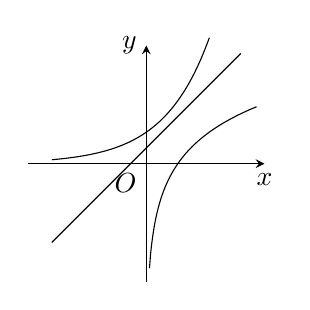
\begin{tikzpicture}[>=stealth,samples=100]
	\draw [->] (-1.5,0)--(0,0) node [below left] {$O$}--(1.5,0) node [below] {$x$};
	\draw [->] (0,-1.5)--(0,1.5) node [left] {$y$};
	\draw [domain=-3:3] plot ({\x*0.4},{(\x+0.5)*0.4});
	\draw [domain=-3:2] plot ({\x*0.4},{exp(\x*ln(2))*0.4});
	\draw [domain=0.1:3.5] plot ({\x*0.4},{ln(\x)/ln(2)*0.4});
	\end{tikzpicture}}{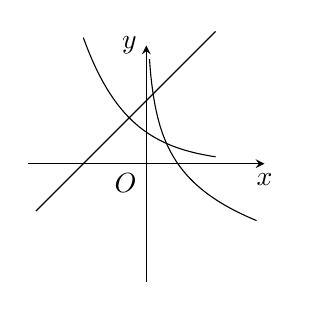
\begin{tikzpicture}[>=stealth,samples=100]
	\draw [->] (-1.5,0)--(0,0) node [below left] {$O$}--(1.5,0) node [below] {$x$};
	\draw [->] (0,-1.5)--(0,1.5) node [left] {$y$};
	\draw [domain=-3.5:2.2] plot ({\x*0.4},{(\x+2)*0.4});
	\draw [domain=-2:2.2] plot ({\x*0.4},{exp(\x*ln(1/2))*0.4});
	\draw [domain=0.1:3.5] plot ({\x*0.4},{-ln(\x)/ln(2)*0.4});
	\end{tikzpicture}}{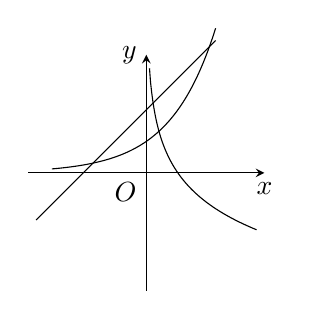
\begin{tikzpicture}[>=stealth,samples=100]
	\draw [->] (-1.5,0)--(0,0) node [below left] {$O$}--(1.5,0) node [below] {$x$};
	\draw [->] (0,-1.5)--(0,1.5) node [left] {$y$};
	\draw [domain=-3.5:2.2] plot ({\x*0.4},{(\x+2)*0.4});
	\draw [domain=-3:2.2] plot ({\x*0.4},{exp(\x*ln(2))*0.4});
	\draw [domain=0.1:3.5] plot ({\x*0.4},{-ln(\x)/ln(2)*0.4});
	\end{tikzpicture}}{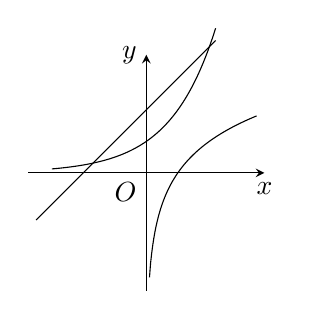
\begin{tikzpicture}[>=stealth,samples=100]
	\draw [->] (-1.5,0)--(0,0) node [below left] {$O$}--(1.5,0) node [below] {$x$};
	\draw [->] (0,-1.5)--(0,1.5) node [left] {$y$};
	\draw [domain=-3.5:2.2] plot ({\x*0.4},{(\x+2)*0.4});
	\draw [domain=-3:2.2] plot ({\x*0.4},{exp(\x*ln(2))*0.4});
	\draw [domain=0.1:3.5] plot ({\x*0.4},{ln(\x)/ln(2)*0.4});
	\end{tikzpicture}}

\item (理科)如图, 四棱锥$S-ABCD$的底面为正方形, $SD\perp $底面$ABCD$, 则下列结论中{\bf 不正确}的是\blank{30}
\twoch{$AC\perp SB$}{$AB\parallel$平面$SCD$}{$AB$与$SC$所成的角等于$DC$与$SA$所成的角}{$SA$与平面$SBD$所成的角等于$SC$与平面$SBD$所成的角}\\
(文科)如图, 在四面体$A-BCD$中, 截面$PQMN$是正方形, $PQ\parallel AC$, $QM\parallel BD$, 则下列命题中, 正确的有\blank{30}.

\textcircled{1} $AC\perp BD$; \textcircled{2} $AC\parallel$截面$PQMN$; \textcircled{3} $AC=BD$; \textcircled{4} 异面直线$PM$与$BD$所成的角为$45^\circ$.
\fourch{\textcircled{1}\textcircled{2}\textcircled{3}}{\textcircled{1}\textcircled{3}\textcircled{4}}{\textcircled{1}\textcircled{2}\textcircled{4}}{\textcircled{2}\textcircled{3}\textcircled{4}}

\begin{center}
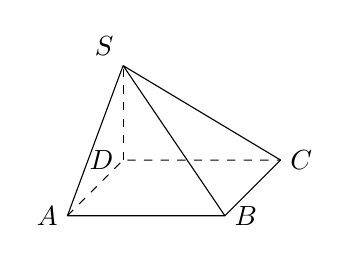
\begin{tikzpicture}
\draw (0,0) node [left] {$A$} coordinate (A)--(2,0) node [right] {$B$} coordinate (B)--({2+0.5*sqrt(2)},{0.5*sqrt(2)}) node [right] {$C$} coordinate (C);
\draw [dashed] (A)--({0.5*sqrt(2)},{0.5*sqrt(2)}) node[left]{$D$} coordinate (D)--(C);
\draw [dashed] (D)--+(0,1.2) node[above left] {$S$} coordinate (S);
\draw (S)--(A) (S)--(B) (S)--(C);
\end{tikzpicture}
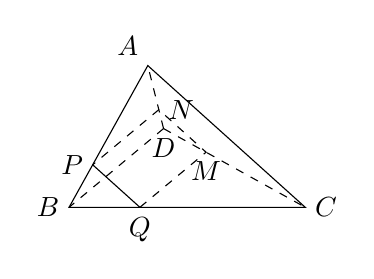
\begin{tikzpicture}
\draw (0,0) coordinate (B) node[left]{$B$}--(3,0) coordinate (C) node [right] {$C$}--(1,1.8) node [above left] {$A$} coordinate (A)--cycle;
\draw [dashed] (1.2,1) node [below]{$D$} coordinate (D)--(A) (D)--(B) (D)--(C);
\coordinate (P) at ($(A)!0.7!(B)$);
\coordinate (Q) at ($(C)!0.7!(B)$);
\coordinate (M) at ($(C)!0.7!(D)$);
\coordinate (N) at ($(A)!0.7!(D)$);
\draw (P) node [left] {$P$}--(Q) node [below] {$Q$};
\draw [dashed] (Q)--(M) node [below] {$M$} --(N) node [right] {$N$} --(P);
\end{tikzpicture}
\end{center}


\newpage

\item 观察下列等式: 

\textcircled{1} $\cos 2\alpha=2\cos^2\alpha-1$; \textcircled{2} $\cos 4\alpha=8\cos^4\alpha-8\cos^2\alpha+1$; \textcircled{3} $\cos 6\alpha=32\cos^6\alpha-48\cos^4\alpha+18\cos^2\alpha-1$; \textcircled{4} $\cos 8\alpha=128\cos^8\alpha-256\cos^6\alpha+160\cos^4\alpha-32\cos^2\alpha+1$ \textcircled{5} $\cos10\alpha=m\cos^{10}\alpha-1280\cos^8\alpha+1120\cos^6\alpha+n\cos^4\alpha+p\cos^2\alpha-1$.
由此可以推测$m-n+p=$\blank{30}.
\fourch{$962$}{$963$}{$964$}{$965$}
\item 已知$P=\{x|x^2-8x-20\le 0\}$, $S=\{x|1-m\le x\le 1+m\}$.\\
(1) 是否存在实数$m$, 使$x\in P$是$x\in S$的充要条件, 若存在, 求出$m$的范围;\\
(2) 是否存在实数$m$, 使$x\in P$是$x\in S$的必要条件, 若存在, 求出$m$的范围.
\item 已知圆$C_1: \left(x+\dfrac{\sqrt{6}}{2}\right)^2+y^2=\dfrac{25}{8}$, 圆$C_2: \left(x-\dfrac{\sqrt{6}}{2}\right)^2+y^2=\dfrac{1}{8}$. 动圆$P$与已知两圆都外切.\\
(1) 求动圆的圆心$P$的轨迹$E$的方程;\\
(2) 直线$l: y=kx+1$与点$P$的轨迹$E$交于不同的两点$A,B$, $AB$的中垂线与$y$轴交于点$N$, 求点$N$的纵坐标的取值范围.
\item 已知向量$\overrightarrow{a}=(1,k)$, $\overrightarrow{b}=(2,2)$, 若$\overrightarrow{a}+\overrightarrow{b}$与$\overrightarrow{a}$共线, 计算$\overrightarrow{a}\cdot\overrightarrow{b}=$\blank{50}.
\item 复数$\dfrac{m+\mathrm{i}}{1+\mathrm{i}}-\dfrac 12$的实部与虚部相等, 则实数$m$的值为\blank{50}.
\item 若$\displaystyle\lim_{n\to \infty}\left(\dfrac{an^2+cn+2}{2n+1}-n\right)=3$, 则$a+c=$\blank{50}.
\item 已知关于$x,y$的二元一次方程组的增广矩阵为$\begin{pmatrix}2 & 3 & 1 \\1 & 1 & 2\end{pmatrix}$, 则$D_x=$\blank{50}.
\item 若$\theta$是某三角形的内角且$\cos2\theta+3\cos\theta+1=0$, 则$\theta=$\blank{50}.
\item (理科)有$3$位射击手独立瞄准一个相同目标, 他们命中的概率都是$0.8$, 则目标恰好被两名射手命中的概率是\blank{50}.\\
(文科)袋子中有大小形状相同的$4$个红球, $3$个白球, 某人随机抽出两个球, 则恰好是一红一白的概率是\blank{50}.
\item 已知$F_1,F_2$为椭圆$\dfrac{x^2}{25}+\dfrac{y^2}{16}=1$的左、右焦点, $P$为椭圆上一点, $M$是$F_1P$的中点, $|OM|=3$, 则点$M$到椭圆左焦点的距离为\blank{50}.
\item (理科)正三棱锥$P-ABC$中, 点$P,A,B,C$都在半径为$\sqrt{3}$的球面上, 若$PA,PB,PC$两两互相垂直, 则球心到截面$ABC$的距离为\blank{50}.
\item 已知正数$x,y$满足$\ln x+\ln y=\ln (x+y)$, 则$2x+y$的最小值是\blank{50}.
\item 二维空间中圆的一维测度(周长)$l=2\pi r$, 二维测度(面积)$S=\pi r^2$; 三维空间中球的二维测度(表面积)$S=4\pi r^2$, 三维测度(体积)$V=\dfrac 43\pi r^3$; 类比观察, 则四维空间中``超球''的三维测度$V=8\pi r^3$, 猜想其四维测度$W=$\blank{50}.
\item 设$l,m,n$是直线, 其中$m,n$在平面$\alpha$内, 则``$l\perp \alpha$''是``$l\perp m, \ l\perp n$''的\blank{30}.
\twoch{充分不必要条件}{必要不充分条件}{充要条件}{既不充分也不必要条件}
\item 方程$(2x+3y-1)(\sqrt{x-3}-1)=0$表示的曲线是\blank{30}.
\fourch{两条直线}{两条射线}{两条线段}{一条直线和一条射线}
\item 已知等比数列$\{a_n\}$的公比$q<0$, 其前$n$项和为$S_n$, 则$a_9S_8$与$a_8S_9$的大小关系是\blank{30}.
\twoch{$a_9S_8>a_8S_9$}{$a_9S_8<a_8S_9$}{$a_9S_8\ge a_8S_9$且可能取到等号}{$a_9S_8\le a_8S_9$且可能取到等号}
\item 已知正数$a,b,c,d$满足$ac\ne bd$. 求证: $\dfrac{a+d}{b+c}$在$\dfrac ab$与$\dfrac dc$之间.
\item 已知$\{a_n\}$为无穷等比数列, 数列$\{b_n\}$满足$b_1+b_2+\cdots+b_n=\dfrac{n}{n+1} \ (n\in \mathbf{N}^*)$, 且$a_1+3b_2=2$, $\displaystyle_{n\to \infty}(a_1+a_2+a_3+\cdots+a_n)=\dfrac 56$. \\
(1) 求数列$\{a_n\}$和$\{b_n\}$的通项公式;\\
(2) 是否存在$m\in \mathbf{N}^*$, 使得当正整数$n\ge m$时, 总有$a_n<b_n$? 若有, 求出$m$的最小值; 若没有, 请说明理由.
\item 若集合$A=\{x||x-2|\le 2\}$, $B=\{y|y=-x^2, \ -1\le x\le 2\}$, 则$A\cap B=$\blank{50}.
\item 若$z_1,z_2$是方程$z^4=4$的两个虚根, 则$z_1\cdot z_2=$\blank{50}.
\item 若抛物线$y^2=2mx$的焦点与双曲线$\dfrac{x^2}{2}-\dfrac{y^2}{2}=1$的右焦点重合, 则$m=$\blank{50}.
\item 已知函数$f(x)=\begin{cases}
\dfrac 3x, & x\ge 3,\\ \log_3 x, & 0<x<3,
\end{cases}$ 若关于$x$的方程$f(x)=k$有两个不同的实根, 则实数$k$的取值范围是\blank{50}.
\item 方程$\dfrac{\sin x}{1+\cos x}=\dfrac{1-\cos x}{\sin x}$的解集为\blank{50}.
\item 若$(1+x)^n+\left(1+x^\frac 12\right)^n+\left(1+x^\frac 13\right)^n+\cdots+\left(1+x^\frac 1n\right)^n \ (n\in \mathbf{N}^*)$的展开式中$x$的系数是$a_n$, 展开式中所有项的系数和为$b_n$, 则$\displaystyle\lim_{n\to \infty}\dfrac{na_n}{b_n}=$\blank{50}.
\item 如图, $M$是平行四边形$ABCD$的边$AB$的中点, 直线$l$过点$M$分别交$AD,AC$于点$E,F$. 若$\overrightarrow{AD}=3\overrightarrow{AE}$, 则$AF:FC=$\blank{50}.
\begin{center}
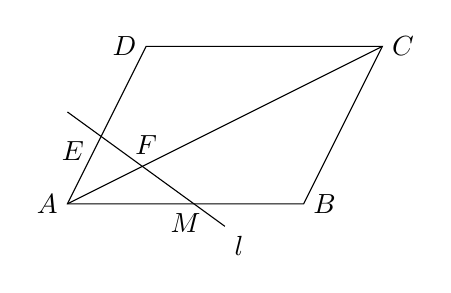
\begin{tikzpicture}
\draw (0,0) node [left] {$A$}--(3,0) node [right] {$B$}--(4,2) node [right] {$C$}--(1,2) node [left] {$D$}--cycle;
\draw (0,0)--(4,2);
\draw (0,{7/6})--(2,{-2/7}) node [below right] {$l$};
\draw ({3/2},0) node [below] {$M$} ({1/3},{2/3}) node [left] {$E$} (1,0.5) node [above] {$F$};
\end{tikzpicture}
\end{center}


\item (理科)某学生在参加政、史、地三门课程的学业水平考试中, 取得A等级的概率分别为$\dfrac 45$, $\dfrac 35$, $\dfrac 25$, 且三门课程的成绩是否取得A等级相互独立. 记$\xi$为该生取得A等级的课程数, 则数学期望$E\xi$的值为\blank{50}.
\item 已知公比为$q(q>0)$的等比数列$\{a_n\}$中, $a_1=256$, 记$\prod_n=a_1\times a_2\times \cdots\times a_n$(即$\prod _n$表示数列$\{a_n\}$的前$n$项之积), 若$\{\prod_n\}$中最大项有且只有$\prod_9$, 则$q$的取值范围是\blank{50}.
\item (理科)一质点从所有棱长都为$1$的正五棱柱$ABCDE-A_1B_1C_1D_1E_1$的顶点$E$出发, 沿正五棱柱的棱运动, 每过一条棱称为一次运动. 运动方向是$E\to A\to B\to B_1\to \cdots$, 从开始在$EA$上称为第$1$棱运动, $AB$上称为第$2$棱运动, $BB_1$上称为第$3$棱运动, $\cdots$, 且第$n+2$棱运动所在棱与第$n$棱运动所在棱是异面直线. 经过$2014$次运动后, 质点到达顶点位置时\blank{50}.\\
(文科)质点从正方体$ABCD-A_1B_1C_1D_1$的顶点$A$出发, 沿正方体的棱运动. 每经过一条棱称为一次运动. 第一次从$A$到$B$, 第二次从$B$到$C$, 运动规律满足第$n+2$次运动所在棱与第$n$次运动所在棱成异面直线. 那么质点经$2014$次运动后到达顶点位置为\blank{50}.
\item 为了从甲乙两人中选一人参加数学竞赛,老师将两人最近的$6$次数学测试的分数进行统计, 甲乙两人的得分情况如下表所示, 
\begin{center}
\begin{tabular}{|c|c|c|c|c|c|c|}
	\hline
	甲 & $72$ & $78$ & $79$ & $85$ & $86$ & $92$\\ \hline
	乙 & $78$ & $86$ & $88$ & $88$ & $91$ & $93$\\ \hline
\end{tabular}
\end{center}
若甲乙两人的平均成绩分别是$\bar{x}_{\text{甲}}$, $\bar{x}_{\text{乙}}$, 则下列说法正确的是\blank{30}.
\twoch{$\bar{x}_{\text{甲}}>\bar{x}_{\text{乙}}$, 乙比甲成绩稳定, 应该选乙参加比赛}{$\bar{x}_{\text{甲}}>\bar{x}_{\text{乙}}$, 甲比乙成绩稳定, 应该选甲参加比赛}{$\bar{x}_{\text{甲}}<\bar{x}_{\text{乙}}$, 甲比乙成绩稳定, 应该选甲参加比赛}{$\bar{x}_{\text{甲}}<\bar{x}_{\text{乙}}$, 乙比甲成绩稳定, 应该选乙参加比赛}
\item 已知$m,n$是两条不同直线, $\alpha,\beta,\gamma$是三个不同平面, 下列命题中正确的是\blank{30}.
\twoch{$m\parallel \alpha$, $n\parallel \alpha$, 则$m\parallel n$}{若$m\parallel \alpha$, $m\parallel \beta$, 则$\alpha\parallel \beta$}{若$\alpha\perp \gamma$, $\beta\perp \gamma$, 则$\alpha\parallel \beta$}{若$m\perp \alpha$, $n\perp \alpha$, 则$m\parallel n$}
\item 平面四边形$ABCD$中, $\overrightarrow{AB}+\overrightarrow{CD}=\overrightarrow{0}$, $(\overrightarrow{AB}-\overrightarrow{AD})\cdot \overrightarrow{AC}=0$, 则四边形$ABCD$是\blank{30}.
\fourch{矩形}{菱形}{等腰梯形}{直角梯形}
\item 已知函数$f(x)=x\begin{vmatrix}
\mathrm{e}^{2x} & 1\\-\mathrm{e}^x & a
\end{vmatrix}$, 其中$\mathrm{e}$是自然对数的底数, $a\in \mathbf{R}$.\\
(1) 当$-1<a<0$时, 解不等式$f(x)<0$;\\
(2) 当$a=0$时, 求整数$t$的所有值, 使方程$f(x)=x+2$在$[t,t+1]$上有解.
\item 如图是一个算法的流程图.\\
(1) 写出数列$\{a_n\}$的前$6$项;\\
(2) 试求输出$S$的值.

\begin{center}
\begin{tikzpicture}[>=stealth]
\draw (-0.5,0) arc (270:90:0.3)--(0.5,0.6) arc (90:-90:0.3) --cycle;
\draw (0,0.3) node {开始};
\draw [->] (0,0)--(0,-0.6);
\draw (-1.2,-0.6) rectangle (1.2,-1.2);
\draw (0,-0.9) node {$i=1, \ S=0$};
\draw [->] (0,-1.2)--(0,-1.8);
\draw (-1.5,-1.8) rectangle (1.5,-2.7);
\draw (0,-2.25) node {$a_i=i\cos\dfrac{i\pi}{2}+1$};
\draw [->] (0,-2.7)--(0,-3.3);
\draw (-1.2,-3.3) rectangle (1.2,-3.9);
\draw (0,-3.6) node {$S=S+a_i$};
\draw [->] (0,-3.9)--(0,-4.5);
\draw (0,-4.5)--(-1.2,-5)--(0,-5.5)--(1.2,-5)--cycle;
\draw (0,-5) node {$i<2014$};
\draw [->] (0,-5.5)--(0,-6.1);
\draw (0,-5.8) node [left] {否};
\draw [->] (1.2,-5) node [above right] {是} -- (3.2,-5)--(3.2,-3.9);
\draw (2,-3.9) rectangle (4.4,-3.3);
\draw (3.2,-3.6) node {$i=i+1$};
\draw [->] (3.2,-3.3)--(3.2,-1.5)--(0,-1.5);
\draw (-0.6,-6.1)--(1,-6.1)--(0.6,-6.7)--(-1,-6.7)--cycle (0,-6.4) node {输出$S$};
\draw [->] (0,-6.7)--(0,-7.3);
\draw (-0.5,-7.9) arc (270:90:0.3)--(0.5,-7.3) arc (90:-90:0.3) --cycle;
\draw (0,-7.6) node {结束};
\end{tikzpicture}
\end{center}
\item 设$\dfrac{\sqrt{3}-\tan\left(\dfrac{\pi}{3}-\theta\right)}{1+\sqrt{3}\tan\left(\dfrac{\pi}{3}-\theta\right)}=3$, 则$\cos 2\theta$等于\blank{50}.
\item 在$(1+x)^n$的展开式中, 第十项是使得二项式系数最大的唯一的项, 则$n$的值是\blank{50}.
\item 光线每穿过一块玻璃板, 其强度就要损失$10\%$, 要使光线的强度减弱到原来的$\dfrac 13$以下, 那么至少需要重叠\blank{50}块玻璃板.
\item 若$|\overrightarrow a|=10$, $\overrightarrow b=(3,-4)$, 且$\overrightarrow a$与$\overrightarrow b$的方向相同, 则$\overrightarrow a=$\blank{50}.
\item 不等式$\lg(-x)<x+1$的解集为\blank{50}.
\item 某科技小组有$6$名同学, 现从中选出$3$人去参观展览, 至少有$1$名女生入选时的不同选法有$16$中, 则小组中的女生人数为\blank{50}.
\item 若用边长为$4$的正方形纸片制作一个母线长为$4$的无底圆锥, 则这样制作出的圆锥的最大体积为\blank{50}.
\item 已知$f(x)=\begin{cases}
1, & x\ge 0,\\-1, & x<0,
\end{cases}$ 则不等式$x+(x+2)f(x+2)\le 5$的解集是\blank{50}.
\item 椭圆$\dfrac{x^2}{a^2}+\dfrac{y^2}{b^2}=1 \ (a>b>0)$和圆$x^2+y^2=\left(\dfrac b2+c\right)^2 \ (c^2=a^2-b^2)$有两个不同的公共点, 则$\dfrac ca$的值是\blank{50}.
\item 设数列$\{a_n\}$为$\dfrac 12,\dfrac 13+\dfrac 23,\dfrac 14+\dfrac 24+\dfrac 34,\cdots$, 若$b_n=\dfrac{1}{a_na_{n+1}}$, 记$\{b_n\}$的前$n$项和为$S_n$, 则$S_{11}$的值为\blank{50}.
\item 若集合$M=\{y|y=x^2-1, \ x\in \mathbf{R}\}$, 集合$N=\{x|y=\sqrt{3-x}, \ x\in \mathbf{R}\}$, 则$M\cap N=$\blank{30}.
\fourch{$\{(-\sqrt{2},1),(\sqrt{2},1)\}$}{$\{t|0\le t\le \sqrt{3}\}$}{$\{t|-1\le t\le 3\}$}{$\{t|-\infty<t\le \sqrt{3}\}$}
\item 设$A(-1,0)$, $B(1,0)$, 条件甲: $A,B,C$是以$C$为直角顶点的三角形的三个顶点; 条件乙: $C$的坐标是方程$x^2+y^2=1$的解, 则甲是乙的\blank{30}.
\fourch{充分非必要条件}{必要非充分条件}{充要条件}{既不充分又不必要条件}
\item 如图, 直角梯形$OABC$中, $AB\parallel OC$, $AB=1$, $OC=BC=2$, 直线$l: x=t$截此梯形所得位于$l$左方图形面积为$S$, 
\begin{center}
	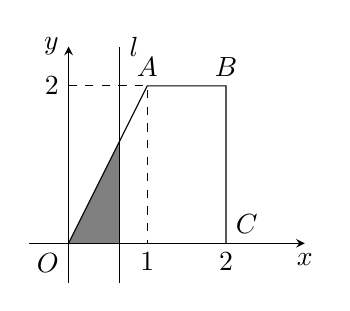
\begin{tikzpicture}[samples=200,>=stealth]
	\fill [gray] (0,0)--(0.65,0)--(0.65,1.3)--cycle;
	\draw [->] (-0.5,0)--(0,0) node [below left] {$O$} --(3,0) node [below] {$x$};
	\draw [->] (0,-0.5)--(0,2.5) node [left] {$y$};
	\draw (0,0)--(1,2) node [above] {$A$}--(2,2) node [above] {$B$}--(2,0) node [above right] {$C$};
	\draw (0.65,-0.5)--(0.65,2.5) node [right] {$l$};
	\draw [dashed] (0,2) node [left] {$2$} --(1,2)--(1,0) node [below] {$1$};
	\draw (2,0) node [below] {$2$};
	
	\end{tikzpicture}
\end{center}
则函数$S=f(t)$的图像大致为\blank{30}.

\fourch{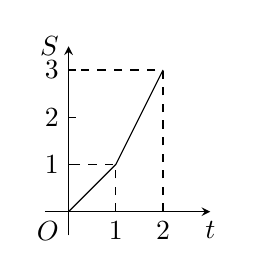
\begin{tikzpicture}[>=stealth]
	\draw [->] (-0.3,0)--(0,0) node [below left] {$O$} --(1.8,0) node [below] {$t$};
	\draw [->] (0,-0.3)--(0,2.1) node [left] {$S$};
	\draw (0.6,0) node [below] {$1$}--(0.6,0.1);
	\draw (1.2,0) node [below] {$2$}--(1.2,0.1);
	\draw (0,0.6) node [left] {$1$}--(0.1,0.6);
	\draw (0,1.2) node [left] {$2$}--(0.1,1.2);
	\draw (0,1.8) node [left] {$3$}--(0.1,1.8);
	\draw (0,0)--(0.6,0.6)--(1.2,1.8);
	\draw [dashed] (0.6,0)--(0.6,0.6)--(0,0.6);
	\draw [dashed] (1.2,0)--(1.2,1.8)--(0,1.8);
	\end{tikzpicture}}{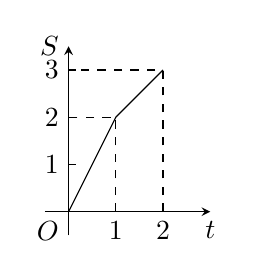
\begin{tikzpicture}[>=stealth]
	\draw [->] (-0.3,0)--(0,0) node [below left] {$O$} --(1.8,0) node [below] {$t$};
	\draw [->] (0,-0.3)--(0,2.1) node [left] {$S$};
	\draw (0.6,0) node [below] {$1$}--(0.6,0.1);
	\draw (1.2,0) node [below] {$2$}--(1.2,0.1);
	\draw (0,0.6) node [left] {$1$}--(0.1,0.6);
	\draw (0,1.2) node [left] {$2$}--(0.1,1.2);
	\draw (0,1.8) node [left] {$3$}--(0.1,1.8);
	\draw (0,0)--(0.6,1.2)--(1.2,1.8);
	\draw [dashed] (0.6,0)--(0.6,1.2)--(0,1.2);
	\draw [dashed] (1.2,0)--(1.2,1.8)--(0,1.8);
	\end{tikzpicture}}{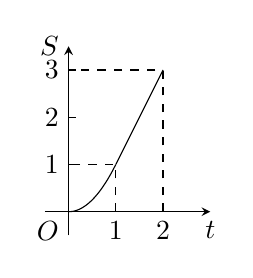
\begin{tikzpicture}[>=stealth,samples=200]
	\draw [->] (-0.3,0)--(0,0) node [below left] {$O$} --(1.8,0) node [below] {$t$};
	\draw [->] (0,-0.3)--(0,2.1) node [left] {$S$};
	\draw (0.6,0) node [below] {$1$}--(0.6,0.1);
	\draw (1.2,0) node [below] {$2$}--(1.2,0.1);
	\draw (0,0.6) node [left] {$1$}--(0.1,0.6);
	\draw (0,1.2) node [left] {$2$}--(0.1,1.2);
	\draw (0,1.8) node [left] {$3$}--(0.1,1.8);
	\draw [domain=0:1] plot ({\x*0.6},{\x*\x*0.6});
	\draw (0.6,0.6)--(1.2,1.8);
	\draw [dashed] (0.6,0)--(0.6,0.6)--(0,0.6);
	\draw [dashed] (1.2,0)--(1.2,1.8)--(0,1.8);
	\end{tikzpicture}}{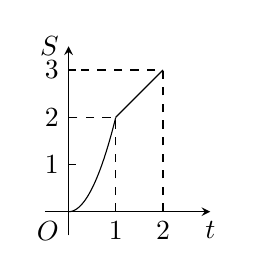
\begin{tikzpicture}[>=stealth,samples=200]
	\draw [->] (-0.3,0)--(0,0) node [below left] {$O$} --(1.8,0) node [below] {$t$};
	\draw [->] (0,-0.3)--(0,2.1) node [left] {$S$};
	\draw (0.6,0) node [below] {$1$}--(0.6,0.1);
	\draw (1.2,0) node [below] {$2$}--(1.2,0.1);
	\draw (0,0.6) node [left] {$1$}--(0.1,0.6);
	\draw (0,1.2) node [left] {$2$}--(0.1,1.2);
	\draw (0,1.8) node [left] {$3$}--(0.1,1.8);
	\draw [domain=0:1] plot ({\x*0.6},{2*\x*\x*0.6});
	\draw (0.6,1.2)--(1.2,1.8);
	\draw [dashed] (0.6,0)--(0.6,1.2)--(0,1.2);
	\draw [dashed] (1.2,0)--(1.2,1.8)--(0,1.8);
	\end{tikzpicture}}

\item 求证: (1) 在所有周长相同的长方形中, 只有正方形的面积最大;\\
(2) 在所有面积相同的长方形中, 只有正方形的面积最小.
\item 平面上定点$F$到定直线$l$的距离$|FM|=2$, $P$为该平面上的动点, 过$P$作直线$l$的垂线, 垂足为$Q$, 且$(\overrightarrow{PF}+\overrightarrow{PQ})\cdot (\overrightarrow{PF}-\overrightarrow{PQ})=0$.\\
(1) 试建立适当的平面直角坐标系, 求动点$P$的轨迹$C$的方程;\\
(2) 过点$F$的直线交轨迹$C$于$A,B$两点, 交直线$l$于点$N$, 已知$\overrightarrow{NA}=\lambda_1\overrightarrow{AF}$, $\overrightarrow{NB}=\lambda_2\overrightarrow{BF}$, 求证: $\lambda_1+\lambda_2$为定值.
\item 集合$\{y|y=2^{-x}\}\cap\{y|y=\lg x, \ 0<x<100\}=$\blank{50}.
\item 若$(1+\mathrm{i})z=a+\mathrm{i}$, $z$对应点在第二象限, 实数$a$的取值范围为\blank{50}.
\item 如果$\left(\dfrac{1}{\sqrt{x}}-\dfrac{\sqrt{2}}{2}\right)^n$展开式第三项的二项式系数为$66$, 那么展开式第六项为\blank{50}.
\item 已知$\sin x=\cos 2x, \ x\in\left(\dfrac{\pi}{2},\pi\right)$, 则$\tan x=$\blank{50}.
\item 函数$f(x)=a^x+b \ (a>1, \ b<-1)$, 则$y=f^{-1}(x)$的图像一定不经过第\blank{50}象限.
\item 函数$f(x)=3\sin (\omega x), \ omega>0$在区间$\left[-\dfrac{\pi}{3},\dfrac{\pi}{4}\right]$单调递增, 则$\omega$的取值范围为\blank{50}.
\item $\triangle OAB$中$OA=3$, $OB=4$, $C$是$AB$中点, 则$\overrightarrow OC\cdot \overrightarrow{AB}=$\blank{50}.
\item 若$\{a,b\}\subseteq \{0,1,2,3,4,5,6\}$, 从复数$a+b\mathrm{i} \ (a\ne b)$中任取一个, 模小于等于$5$的概率为\blank{50}.
\item (理科)一个不透明的袋中装有白球、红球共$9$个($9$个球除颜色外其余完全相同), 经充分混合后, 从袋中随机摸出$2$球, 且摸出的$2$球中至少有一个是白球的概率为$\dfrac 56$, 现用$\xi$表示摸出的$2$个球中红球的个数, 则随机变量$\xi$的数学期望$E\xi=$\blank{50}.\\
(文科)一个不透明的袋中装有$5$个白球、$4$个红球($9$个球除颜色外其余完全相同), 经充分混合后, 从袋中随机摸出$3$球, 则摸出的$3$球中至少有一个是白球的概率为\blank{50}.
\item 已知数列$\{a_n\}$的通项$a_n=\left(\dfrac 13\right)^n$, 数列$\{b_n\}$满足$b_1=-1$, $b_2=2$, $b_{n+2}=b_n, \ n\in \mathbf{N}^*$, 则$\displaystyle\lim_{n\to \infty}(a_1b_1+a_2b_2+\cdots+a_nb_n)=$\blank{50}.
\item 在长方体$ABCD-A_1B_1C_1D_1$中, $B_1C$和$C_1D$与底面所成的角分别为$60^\circ$和$45^\circ$, 则异面直线$B_1C$和$C_1D$所成的角的余弦值为\blank{30}.
\fourch{$\dfrac{\sqrt{3}}6$}{$\dfrac{\sqrt{2}}{6}$}{$\dfrac{\sqrt{6}}{3}$}{$\dfrac{\sqrt{6}}{4}$}
\item (理科)甲、乙、丙、丁与小强一起比赛象棋, 每两人都要比赛一盘, 到现在为止, 甲已经赛了$4$盘, 乙赛了$3$盘, 丙赛了$2$盘, 丁赛了$1$盘, 则小强已经赛了\blank{30}.
\fourch{$4$盘}{$3$盘}{$2$盘}{$1$盘}\\
(文科)``$-2\le a\le 2$''是``实系数一元二次方程$x^2+ax+1=0$有虚根''的\blank{30}.
\fourch{充要条件}{必要不充分条件}{充分不必要条件}{既不充分也不必要条件}
\item 已知点$P(x,y)$是直线$kx+y+4=0 \ (k>0)$上一动点, $PA,PB$是圆$C:x^2+y^2-2y=0$的两条切线, $A,B$是切点, 若四边形$PACB$($C$为圆心)面积的最小值为$2$, 则$k$的值为\blank{30}.
\fourch{$2$}{$\dfrac{\sqrt{21}}{2}$}{$2\sqrt{2}$}{$3$}
\item 已知$\triangle ABC$的面积为$3$, 且满足$0\le \overrightarrow{AB}\cdot\overrightarrow{AC}\le 6$, 设$\overrightarrow{AB}$和$\overrightarrow{AC}$的夹角为$\theta$.\\
(1) 求$\theta$的取值范围;\\
(2) 求函数$f(\theta)=2\sin^2\left(\dfrac{\pi}{4}+\theta\right)-\sqrt{3}\cos 2\theta$的最大值与最小值.
\item (理科)在底面是直角梯形的四棱锥$S-ABCD$中, $\angle ABC=90^\circ$, $AD\parallel BC$, $SA\perp$平面$ABCD$, $SA=AB=BC=1$, $AD=\dfrac 12$, 求平面$SCD$与平面$SAB$所成的二面角的大小.\\
(文科)如图, 在体积为$\dfrac 13$的三棱锥$P-ABC$中, $PA\perp$平面$ABC$, $\angle ACB=90^\circ$, $PA=2AC=2BC$. 点$M,N$分别是$PB,PC$的中点.\\
(1) 求异面直线$AN$与$CM$所成的角的大小;\\
(2) 求$A$到平面$PBC$的距离.
\begin{center}
	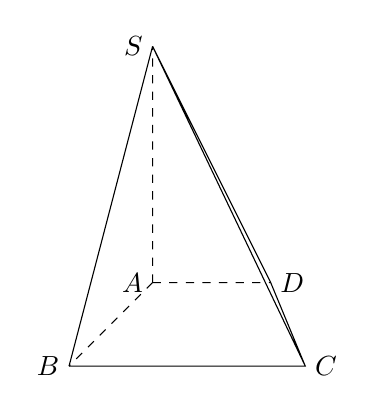
\begin{tikzpicture}
	\coordinate (A) at (0,0);
	\coordinate (D) at (1.5,0);
	\coordinate (B) at ({-sqrt(2)*3/4},{-sqrt(2)*3/4});
	\coordinate (C) at ({-sqrt(2)*3/4+3},{-sqrt(2)*3/4});
	\coordinate (S) at (0,3);
	\draw (B) --(C)--(S)--(D) node [right] {$D$} (S) node [left] {$S$}--(B) node [left] {$B$} (C) node [right] {$C$}--(D);
	\draw [dashed] (A) node [left] {$A$}--(B) (A)--(S) (A)--(D);
	\end{tikzpicture}
\end{center}
\begin{center}
	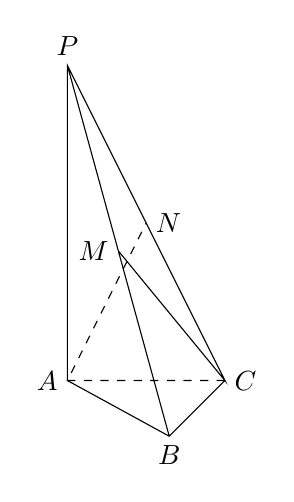
\begin{tikzpicture}
	\coordinate (A) at (0,0);
	\coordinate (C) at (2,0);
	\coordinate (P) at (0,4);
	\coordinate (B) at ({2-sqrt(2)/2},{-sqrt(2)/2});
	\coordinate (M) at ($(B)!0.5!(P)$);
	\coordinate (N) at ($(C)!0.5!(P)$);
	\draw (C) node [right] {$C$}--(B) node [below ] {$B$} --(A) node[left]{$A$}--(P) node [above]{$P$}--(C)--(M) node [left] {$M$} (P)--(B);
	\draw [dashed] (C)--(A)--(N) node [right] {$N$};
	
	\end{tikzpicture}
\end{center}
\item 若$z=\sin\theta-\dfrac 35+\left(\cos\theta-\dfrac 45\right)\mathrm{i}$是纯虚数, 则$\tan\left(\theta-\dfrac{\pi}{4}\right)=$\blank{50}.
\item 要使$y=x^2+4x \ (x\ge a)$有反函数, 则$a$的最小值为\blank{50}.
\item 三个实数成等差数列, 首项是$9$. 若将第二项加$2$, 第三项加$20$可使得这三个数依次构成等比数列$\{a_n\}$, 则$a_3$的所有取值中的最小值是\blank{50}.
\item 二项式$\left(x+\dfrac 1{2x}\right)^8$展开式中的二项式系数最大的项的系数为\blank{50}.
\item 已知函数$y=f(x)$的定义域为$\{x|-3\le x\le 8, \ x\ne 5\}$, 值域为$\{y|-1\le y\le 2, \ y\ne 0\}$. 下列关于函数$y=f(x)$的说法: \textcircled{1} 当$x=-3$时, $y=-1$; \textcircled{2} 将$y=f(x)$的图像补上$(5,0)$, 得到的图像必定是一条连续的曲线; \textcircled{3} $y=f(x)$是$[-3,5)$上的单调函数; \textcircled{4} $y=f(x)$的图像与坐标轴只有一个交点. 其中正确的命题是\blank{50}.
\item 点$P$是双曲线$\dfrac{x^2}{4}-y^2=1$的右支上一点, $M,N$分别是圆$(x+\sqrt{5})^2+y^2=1$和圆$(x-\sqrt{5})^2+y^2=1$上的点, 则$|PM|-|PN|$的最大值是\blank{50}.
\item 设$\triangle ABC$的内角$A,B,C$所对的边分别为$a,b,c$, 若三边的长为连续的三个正整数, 且$A>B>C, \ A=2C$, 则$\sin A:\sin B:\sin C$为\blank{50}.
\item 从集合$\{1,2,3,4,5,6,7,8,9\}$中任取两个不同的数, 则其中一个数恰是另一个数的$3$倍的概率为\blank{50}.
\item 在$\triangle ABC$中, 边$AC=1$, $AB=2$, 角$A=\dfrac{2\pi}{3}$, 过$A$作$AP\perp BC$于$P$, 且$\overrightarrow{AP}=\lambda \overrightarrow{AB}+\mu \overrightarrow{A}$, 则$\lambda\mu=$\blank{50}.
\item 已知函数$f(x)=\begin{cases}ax^2-2x-1, & x\ge 0,\\ x^2+bx+c, & x<0\end{cases}$是偶函数, 直线$y=t$与函数$y=f(x)$的图像自左向右依次交于四个不同点$A,B,C,D$. 若$AB=BC$, 则实数$t$的值为\blank{50}.
\item 直线$\begin{vmatrix}
x & 0 & 1\\-1 & 2 & -1\\y & 1 & 1
\end{vmatrix}=0$的一个法向量是\blank{30}.
\fourch{$(2,3)$}{$(3,-2)$}{$(-2,3)$}{$(3,2)$}
\item 已知平面$\alpha,\beta$和直线$m$, 给出条件: \textcircled{1} $m\parallel \alpha$; \textcircled{2} $m\perp \alpha$; \textcircled{3} $m\subseteq \alpha$; \textcircled{4} $\alpha\perp \beta$; \textcircled{5} $\alpha\parallel\beta$. 由给出的两个条件能推导出$m\parallel \beta$的是\blank{30}.

\fourch{\textcircled{1}\textcircled{4}}{\textcircled{1}\textcircled{5}}{\textcircled{2}\textcircled{4}}{\textcircled{3}\textcircled{5}}
\item 已知函数$f(x)$是定义在$(-\infty,0)\cup (0,+\infty)$上的偶函数, 当$x>0$时, $f(x)=\begin{cases}
2^{|x-1|}-1, & 0<x\le 2,\\\dfrac 12f(x-2), & x>2,
\end{cases}$ 则函数$g(x)=4f(x)-1$的零点的个数为\blank{30}.
\fourch{$4$}{$6$}{$8$}{$10$}
\item 已知圆方程为$x^2+y^2-2ax-4ay+4a^2+t=0 \ (a\ne 0)$.\\
(1) 若$t=\dfrac 12 a^2$, 确定无论$a$为何值均与圆相切的直线的方程;\\
(2) 若$t=a^2-4$, 确定无论$a$为何值被圆截得的弦长为$1$的直线的方程.
\item 对于函数$f(x)=ax^2+(b+1)x+b-2 \ (a\ne 0)$, 若存在实数$x_0$, 使$f(x_0)=x_0$成立, 则称$x_0$为$f(x)$的不动点.\\
(1) 若对于任何实数$b$, 函数$f(x)$恒有两个相异的不动点, 求实数$a$的取值范围;\\
(2) 在(1)的条件下, 若函数$y=f(x)$的图像上$A,B$两点的横坐标是函数$f(x)$的不动点, 且直线$y=kx+\dfrac{1}{2a^2+1}$是线段$AB$的垂直平分线, 求实数$b$的取值范围.
\item 已知椭圆$\dfrac{x^2}{t^2}+\dfrac{y^2}{5t}=1$的焦距为$2\sqrt{6}$, 则实数$t=$\blank{50}.
\item 函数$y=x^2+4x \ (x<-3)$的反函数为\blank{50}.
\item 已知$a$是实数, 若$A=\{x|ax^2+6x+9=0, \ x\in \mathbf{R}\}$中至多有一个元素, 则$a$的取值范围为\blank{50}.
\item 已知球$O$的半径为$4$, $A,B$是球面上两点, $\angle AOB=45^\circ$, 则$A,B$两点的球面距离为\blank{50}.
\item 设$A_n$为$(1+x)^{n+1}$的展开式中含$x^{n-1}$项的系数, $B_n$为$(1+x)^{n-1}$的展开式中二项式系数的和($n\in \mathbf{N}^*$), 则能使$A_n\ge B_n$成立的$n$的最大值是\blank{50}.
\item 已知不等式$a\le \dfrac{x^2+2}{|x|}$对$x$取一切非零实数恒成立, 则$a$的取值范围是\blank{50}.
\item 已知数列$\{a_n\}$是等差数列, 前$n$项和为$S_n$, 若$\overrightarrow{OP}=a_{1006}\overrightarrow{OA}+a_{1009}\overrightarrow{OB}$, 且$P,A,B$三点共线($O$不在该直线上), 则$S_{2014}=$\blank{50}.
\item 已知函数$f(x)=\sin x+\tan \dfrac x2+x^3, \ x\in (-1,1)$, 则满足不等式$f(a-1)+f(2a-1)<0$的实数$a$的取值范围是\blank{50}.
\item 有两个相同的直三棱柱, 高为$\dfrac 2a$, 底面三角形的三边长分别是$3a,4a,5a \ (a>0)$. 用它们拼成一个三棱柱或四棱柱, 在所有可能的情形中, 表面积最小的棱柱只有一种, 是一个三棱柱. 则实数$a$的取值范围是\blank{50}.
\item 设$f(x)=a\sin 2x+b\cos 2x$, 其中$a,b\in \mathbf{R}$, $ab\ne 0$. 若$f(x)\le \left|f\left(\dfrac{\pi}{6}\right)\right|$对一切$x\in \mathbf{R}$恒成立, 则

\textcircled{1} $f\left(\dfrac{11\pi}{12}\right)=0$; \textcircled{2} $\left|f\left(\dfrac{7\pi}{12}\right)\right|<\left|f\left(\dfrac{\pi}{5}\right)\right|$; \textcircled{3} $f(x)$既不是奇函数也不是偶函数; \textcircled{4} $\left[k\pi+\dfrac{\pi}{6},k\pi+\dfrac{2\pi}{3}\right] \ (k\in \mathbf{Z})$是$f(x)$的单调区间; \textcircled{5} 存在经过点$(a,b)$的直线与函数$f(x)$的图像不相交. 

以上结论正确的是\blank{50}(写出所有正确结论的编号).
\item 已知条件$p: |x+1|>2$, 条件$q: x>a$, 且$\bar{p}$是$\bar{q}$的充分不必要条件, 则$a$的取值范围可以是\blank{30}.
\fourch{$a\ge 1$}{$a\le 1$}{$a\ge -1$}{$a\le -3$}
\item 已知$\{a_n\}$是以$a \ (a>0)$为首项以$q \ (-1<q<0)$为公比的等比数列, 设$A=\displaystyle\lim_{n\to \infty}(a_1+a_2+\cdots+a_n)$, $B=\displaystyle\lim_{n\to \infty}(a_1+a_2+a_3\cdots+a_{2n})$, $C=\displaystyle\lim_{n\to \infty}(a_1+a_3+a_5+\cdots+a_{2n-1})$, $D=\displaystyle\lim_{n\to \infty}(a_2+a_4+a_6+\cdots+a_{2n})$. 则$A,B,C,D$的大小关系是\blank{30}.
\fourch{$D<A<B<C$}{$D<A=B<C$}{$C<D<B<A$}{$A=B=C=D$}
\item 设$f(x)$是定义在$\mathbf{R}$上的函数, 且对任意实数$x$, 恒有$f(x+2)=-3f(x)$. 当$x\in [0,2]$时, $f(x)=2x-x^2$, 则$f(0)+f(-1)+f(-2)+\cdots+f(-2014)=$\blank{30}.
\fourch{$-\dfrac 34(1-3^{1007})$}{$-\dfrac 34(1+3^{1007})$}{$-\dfrac 14\left(1-\dfrac{1}{3^{1007}}\right)$}{$-\dfrac 14\left(1+\dfrac{1}{3^{1007}}\right)$}
\item 已知复数$z_1=\sqrt{3}+\mathrm{i}$, $|z_2|=2$, $z_1\cdot z_2^2$是虚部为正数的纯虚数.\\
(1) 求$z_1\cdot z_2^2$的模;\\
(2) 求复数$z_2$.
\item 已知椭圆$C:\dfrac{x^2}{a^2}+\dfrac{y^2}{b^2}=1 \ (a>b>0)$的一个焦点坐标为$(1,0)$, 且长轴长是短轴长的$\sqrt{2}$倍.\\
(1) 求椭圆$C$的方程;\\
(2) 设$O$为坐标原点, 椭圆$C$与直线$y=kx+1$相交于两个不同的点$A,B$, 线段$AB$的中点为$P$, 若直线$OP$的斜率为$-1$, 求$\triangle AOB$的面积.
\item 已知$\sin\alpha=\dfrac 5{13}$, $\alpha\in \left(\dfrac{\pi}{2},\dfrac{3\pi}{2}\right)$, 则$\tan\left(\dfrac{\pi}{4}+\alpha\right)$的值是\blank{50}.
\item 已知函数$f(x)=\begin{cases}
2^x-1, & x\ge 0,\\ -x^2-2x, & x<0,
\end{cases}$ 若$f(a)=1$, 则实数$a$的值是\blank{50}.
\item 已知$x,y\in \mathbf{R}$, 且$x+2y=1$, 则$2^x+4^y$的最小值是\blank{50}.
\item 设点$P(x_0,y_0)$是函数$y=\tan x$与$y=-x \ (x>0)$的图像的一个交点, 则$(x_0^2+1)(\cos 2x_0+1)=$\blank{50}.
\item 投掷一枚质地均匀的骰子两次, 若第一次面向上的点数小于第二次面向上的点数, 我们称其为正实验; 若第二次面上上的点数小于第一次面向上的点数, 我们称其为负实验; 若两次面向上的点数相等, 我们称其为无效实验. 那么一个人投掷该骰子两次后出现无效实验的概率是\blank{50}.
\item 向量$\overrightarrow{a}=(3,-4)$, 向量$\left|\overrightarrow b\right|=2$, 若$\overrightarrow a\cdot \overrightarrow b=-5$, 那么向量$\overrightarrow a$, $\overrightarrow b$的夹角是\blank{50}.
\item 下图所示为一个判断直线$Ax+By+C=0$与圆$(x-a)^2+(y-b)^2=r^2$的位置关系的程序框图的一部分, 在``$?$''处应填上\blank{50}.
\begin{center}
	\begin{tikzpicture}[>=stealth]
	\draw [->] (-0.4,0)--(0,0);
	\draw (-0.3,-0.3)--(0.3,0.3)--(2.7,0.3)--(2.1,-0.3)--cycle;
	\draw (1.2,0) node {输入$A,B,C$};
	\draw [->] (2.4,0)--(2.8,0);
	\draw (2.5,-0.3)--(3.1,0.3)--(5.5,0.3)--(4.9,-0.3)--cycle;
	\draw (4,0) node {输入$a,b,r$};
	\draw [->] (5.2,0)--(5.6,0);
	\draw (5.6,-0.6) rectangle (8.6,0.6);
	\draw (7.1,0) node {$d=\dfrac{|\phantom{11}?\phantom{11}|}{\sqrt{A^2+B^2}}$};
	\draw [->] (8.6,0)--(9,0);
	\draw (9,0)--(10,0.5)--(11,0)--(10,-0.5)--cycle;
	\draw (10,0) node {$d=r$};
	\draw [->] (11,0)--(11.4,0);
	\draw (11.2,0) node [above] {是};
	\draw [->] (10,-0.5)node [below right] {否}--(10,-0.9); 
	\draw (11.1,-0.3)--(11.7,0.3)--(15.1,0.3)--(14.5,-0.3)--cycle;
	\draw (13.2,0) node {输出直线与圆相切};
	\draw[->] (14.8,0)--(15.2,0);
	\end{tikzpicture}
\end{center}

\item 已知曲线$C_1,C_2$的极坐标方程分别为$\rho=4\cos\theta \ \left(\rho\ge 0, \ 0\le \theta<\dfrac{\pi}{2}\right)$, $\rho\cos\theta=3$, 则曲线$C_1$与$C_2$交点的极坐标为\blank{50}.
\item 椭圆两焦点为$F_1(-4,0)$, $F_2(4,0)$, $P$在椭圆上, 若$\triangle PF_1F_2$的面积的最大值为$12$, 则该椭圆的标准方程为\blank{50}.
\item 将正整数按下表的规律排列, 把行与列交叉处的一个数称为某行某列的数, 记作$a_{i,j} \ (i,j\in \mathbf{N}^*)$, 如第$2$行第$4$列的数是$15$, 记作$a_{2,4}=15$, 则$a_{12,14}=$\blank{50}.
\begin{center}
\begin{tabular}{cccccccc}
$1$ & $4$ & $5$ & $16$ & $17$ & $36$ & $\cdots$\\
$2$ & $3$ & $6$ & $15$ & $18$ & $35$ & $\cdots$\\
$9$ & $8$ & $7$ & $14$ & $19$ & $34$ & $\cdots$\\
$10$ & $11$ & $12$ & $13$ & $20$ & $33$ & $\cdots$\\
$25$ & $24$ & $23$ & $22$ & $21$ & $32$ & $\cdots$\\
$26$ & $27$ & $28$ & $29$ & $30$ & $31$ & $\cdots$\\
$\cdots$ & $\cdots$ & $\cdots$ & $\cdots$ & $\cdots$ & $\cdots$ & $\cdots$
\end{tabular}
\end{center}
\item 设矩形的长为$a$, 宽为$b$, 其比满足$b:a=\dfrac{\sqrt{5}-1}{2}\approx 0.618$, 这种矩形给人以美感, 称为黄金矩形. 黄金矩形常应用于工艺品设计中. 下面是某工艺品厂随机抽取两个批次的初加工矩形宽度与长度的比值样本:
\begin{center}
\begin{tabular}{cccccc}
甲批次: & $0.598$ & $0.625$ & $0.628$ & $0.595$ & $0.639$\\
乙批次: & $0.618$ & $0.613$ & $0.592$ & $0.622$ & $0.620$
\end{tabular}
\end{center}
跟据上述两个样本来估计两个批次的总体平均数, 与标准值$0.618$作比较, 正确结论是\blank{30}
\twoch{甲批次的总体平均数与标准值更接近}{甲批次的总体平均数与标准值更接近}{两个批次总体平均数与标准值接近程度相同}{两个批次总体平均数与标准值接近程度不能确定}
\item 已知函数$f(x)=\dfrac{x}{1+|x|} \ (x\in \mathbf{R})$时, 则下列结论{\bf 不正确}的是\blank{30}.
\onech{任意$x\in \mathbf{R}$, 等式$f(-x)+f(x)=0$恒成立}{存在$m\in (0,1)$, 使得方程$|f(x)|=m$有两个不等实数根}{对任意$x_1,x_2\in \mathbf{R}$, 若$x_1\ne x_2$, 则一定有$f(x_1)\ne f(x_2)$}{存在$k\in (1,+\infty)$, 使得函数$g(x)=f(x)-kx$在$\mathbf{R}$上三个零点}
\item 给出下列类比推理命题($\mathbf{R}$为实数集, $\mathbf{C}$为复数集, $M$为平面向量集), 其中类比结论正确的是\blank{30}.
\onech{由``若$a\in \mathbf{R}$, 则$a^2=|a|^2$''类比推出``若$a\in \mathbf{C}$, 则$a^2=|a|^2$''}{由``若$a,b\in \mathbf{R}$, 且$a-b=0$, 则$a=b$''类比推出``若$\overrightarrow{a},\overrightarrow{b}\in \mathbf{M}$, 且$\overrightarrow a-\overrightarrow b=\overrightarrow 0$, 则$\overrightarrow a=\overrightarrow b$''}{由``若$a,b\in \mathbf{R}$, 且$a^2+b^2=0$, 则$a=0$或$b=0$''类比推出``若$a,b\in \mathbf{C}$, 且$a^2+b^2=0$, 则$a=0$或$b=0$''}{由``若$a,b\in \mathbf{R}$, 且$a\cdot b=0$, 则$a=0$或$b=0$''类比推出``若$\overrightarrow a, \overrightarrow b\in \mathbf{M}$, 且$\overrightarrow a\cdot \overrightarrow b=0$, 则$\overrightarrow a=\overrightarrow 0$或$\overrightarrow b=\overrightarrow 0$''}
\item (1) 设$x,y$是不全为零的实数, 试比较$2x^2+y^2$与$x^2+xy$的大小;\\
(2) 设$a,b,c$为正数, 且$a^2+b^2+c^2=1$, 求证: $\dfrac 1{a^2}+\dfrac 1{b^2}+\dfrac 1{c^2}-\dfrac{2(a^3+b^3+c^3)}{abc}\ge 3$.
\item 数列$\{a_n\}$的首项为$1$, 前$n$项和是$S_n$, 存在常数$A,B$使$a_n+S_n=An+B$对任意正整数$n$都成立.\\
(1) 设$A=0$, 求证: 数列$\{a_n\}$是等比数列;\\
(2) 设数列$\{a_n\}$是等差数列, 若$p<q$, 且$\dfrac{1}{S_p}+\dfrac{1}{S_q}=\dfrac{1}{S_{11}}$, 求$p,q$的值;\\
(3) 设$A>0$, $A\ne 1$, 且$\dfrac{a_n}{a_{n+1}}\le M$对任意正整数$n$都成立, 求$M$的取值范围.
\item 已知集合$A=\{x|x^2-2x\le 0 \}$, $B=\{x|-1<x<1\}$, 则$A\cap B=$\blank{50}.
\item 若复数$(1+\mathrm{i})(a+\mathrm{i})$是实数($\mathrm{i}$是虚数单位), 则实数$a$的值\blank{50}.
\item 已知数列$\{a_n\}$是等差数列, 若$a_4+2a_6+a_8=12$, 则该数列前$11$项的和为\blank{50}.
\item 阅读下图的程序框图, 若输入$n=5$, 则输出$k$的值为\blank{50}.
\begin{center}
	\begin{tikzpicture}[>=stealth]
	\draw (0,-0.3)--(1,-0.3) arc (-90:90:0.3)--(0,0.3) arc (90:270:0.3);
	\draw (0.5,0) node {开始};
	\draw [->] (1.3,0)--(1.7,0);
	\draw (1.4,-0.3)--(2,0.3)--(3.6,0.3)--(3,-0.3)--cycle;
	\draw (2.5,0) node {输入$n$};
	\draw [->](3.3,0)--(3.7,0);
	\draw (3.7,0.3) rectangle (4.9,-0.3);
	\draw (4.3,0) node {$k=0$};
	\draw [->] (4.9,0)--(5.3,0);
	\draw (5.3,0.3) rectangle (7.1,-0.3);
	\draw (6.2,0) node {$n=3n+1$};
	\draw [->] (7.1,0)--(7.5,0);
	\draw (7.5,0)--(8.4,0.5)--(9.3,0)--(8.4,-0.5)--cycle;
	\draw (8.4,0) node {$n>150$};
	\draw [->] (9.3,0) --(9.7,0); 
	\draw (9.5,0) node [above]{是};
	\draw [->] (8.4,-0.5) node [below right] {否}--(8.4,-0.9)--(7.1,-0.9);
	\draw (7.1,-1.2) rectangle (5.3,-0.6);
	\draw (6.2,-0.9) node {$k=k+1$};
	\draw [->] (5.3,-0.9)--(3.5,-0.9)--(3.5,0);
	\draw (9.4,-0.3)--(10,0.3)--(11.8,0.3)--(11.2,-0.3)--cycle;
	\draw (10.6,0) node {输出$k,n$};
	\draw [->] (11.5,0)--(11.9,0);
	\draw (12.2,0.3) arc (90:270:0.3)--(13.2,-0.3) arc (-90:90:0.3)--cycle;
	\draw (12.7,0) node {结束};
	\end{tikzpicture}
\end{center}


\item 如图所示, 已知正方体$ABCD-A_1B_1C_1D_1$的棱长为$2$, 长为$2$的线段$MN$的一个端点$M$在棱$DD_1$上运动, 另一端点$N$在正方形$ABCD$内运动, 则$MN$的中点的轨迹的面积为\blank{50}.
\begin{center}
	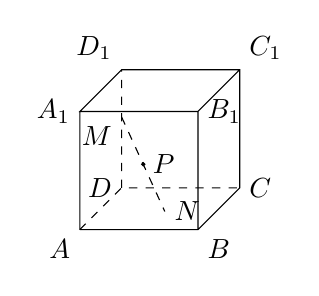
\begin{tikzpicture}
	\draw (0,0) node [below left] {$A$}--(1.5,0) node [below right] {$B$}--({1.5+0.375*sqrt(2)},{0.375*sqrt(2)}) node [right] {$C$}--({1.5+0.375*sqrt(2)},{1.5+0.375*sqrt(2)}) node [above right] {$C_1$}--({0.375*sqrt(2)},{1.5+0.375*sqrt(2)}) node [above left] {$D_1$} --(0,1.5) node [left] {$A_1$}--(1.5,1.5) node [right] {$B_1$}--(1.5,0) (1.5,1.5)--({1.5+0.375*sqrt(2)},{1.5+0.375*sqrt(2)}) (0,0)--(0,1.5);
	\draw [dashed] (0,0)--({0.375*sqrt(2)},{0.375*sqrt(2)}) node [left] {$D$}--({1.5+0.375*sqrt(2)},{0.375*sqrt(2)}) ({0.375*sqrt(2)},{0.375*sqrt(2)})--({0.375*sqrt(2)},{1.5+0.375*sqrt(2)});
	\draw [dashed] ({0.375*sqrt(2)},{0.375*sqrt(2)+0.9}) coordinate (M) node [below left] {$M$}--({0.375*sqrt(2)+0.6*sqrt(2)-0.3},{0.375*sqrt(2)-0.3}) coordinate (N) node [right] {$N$};
	\coordinate (P) at ($(M)!0.5!(N)$);
	\filldraw (P) circle (0.02) node [right] {$P$};
	\end{tikzpicture}
\end{center}


\item 以抛物线$C:y^2=8x$上的一点$A$为圆心作圆, 若该圆经过抛物线$C$的顶点和焦点, 那么该圆的方程为\blank{50}.
\item $\triangle ABC$的三个内角$A,B,C$所对边的长分别为$a,b,c$, 已知$c=3$, $C=\dfrac{\pi}{3}$, $a=2b$, 则$b$的值为\blank{50}.
\item 若函数$y=\cos(\omega x+\varphi) \ (\omega>0, \ 0<\varphi<\pi)$为奇函数, $A,B$分别为相邻的两个最高点, 并且两点间的距离为$4$, 则该函数的图像的对称轴为\blank{50}.
\item 若称横坐标、纵坐标都为整数的点为``整点'', 过曲线$y=\sqrt{100-x^2}$上任意两个整点作直线, 则倾斜角不小于$30^\circ$的直线条数为\blank{50}.
\item 数列$\{a_n\}$满足$a_1=1$, $\sqrt{\dfrac{1}{a_n^2}+4}=\dfrac{1}{a_{n+1}}$, 记数列$\{a_n^2\}$前$n$项的和为$S_n$, 若$S_{2n+1}-S_n\le \dfrac t{30}$对任意的$n\in \mathbf{N}^*$恒成立, 则正整数$t$的最小值为\blank{50}.
\item 设函数$f(x)=\cos^2\left(x+\dfrac{\pi}{4}\right)-\sin^2\left(x+\dfrac{\pi}{4}\right)$, $x\in \mathbf{R}$, 则函数$f(x)$是\blank{30}.
\twoch{最小正周期为$\pi$的奇函数}{最小正周期为$\pi$的偶函数}{最小正周期为$\dfrac{\pi}{2}$的奇函数}{最小正周期为$\dfrac{\pi}{2}$的偶函数}
\item 函数$y=\ln(\cos x) \ \left(-\dfrac{\pi}{2}<x<\dfrac{\pi}{2}\right)$的大致图像是\blank{30}.
\fourch{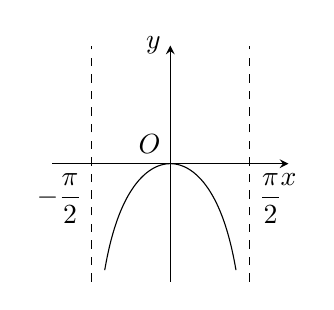
\begin{tikzpicture}[samples=200,>=stealth]
	\draw [->](-1.5,0)--(0,0) node [above left] {$O$}--(1.5,0) node [below] {$x$};
	\draw [->](0,-1.5)--(0,1.5) node [left] {$y$};
	\draw [dashed] (-1,-1.5)--(-1,1.5) (1,-1.5)--(1,1.5);
	\draw (-1,0) node [below left] {$-\dfrac{\pi}{2}$};
	\draw (1,0) node  [below right] {$\dfrac{\pi}{2}$};
	\draw [domain=-75:75] plot ({\x/90},{ln(cos(\x))});
	\end{tikzpicture}}{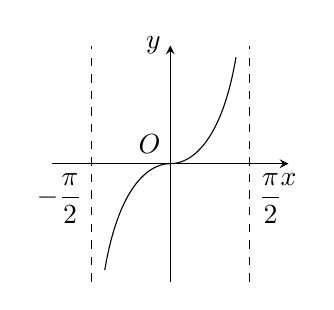
\begin{tikzpicture}[samples=200,>=stealth]
	\draw [->](-1.5,0)--(0,0) node [above left] {$O$}--(1.5,0) node [below] {$x$};
	\draw [->](0,-1.5)--(0,1.5) node [left] {$y$};
	\draw [dashed] (-1,-1.5)--(-1,1.5) (1,-1.5)--(1,1.5);
	\draw (-1,0) node [below left] {$-\dfrac{\pi}{2}$};
	\draw (1,0) node  [below right] {$\dfrac{\pi}{2}$};
	\draw [domain=-75:0] plot ({\x/90},{ln(cos(\x))});
	\draw [domain=0:75] plot ({\x/90},{-ln(cos(\x))});
	\end{tikzpicture}}{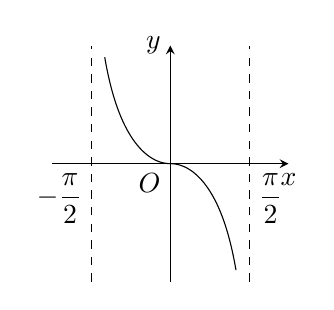
\begin{tikzpicture}[samples=200,>=stealth]
	\draw [->](-1.5,0)--(0,0) node [below left] {$O$}--(1.5,0) node [below] {$x$};
	\draw [->](0,-1.5)--(0,1.5) node [left] {$y$};
	\draw [dashed] (-1,-1.5)--(-1,1.5) (1,-1.5)--(1,1.5);
	\draw (-1,0) node [below left] {$-\dfrac{\pi}{2}$};
	\draw (1,0) node  [below right] {$\dfrac{\pi}{2}$};
	\draw [domain=-75:0] plot ({\x/90},{-ln(cos(\x))});
	\draw [domain=0:75] plot ({\x/90},{ln(cos(\x))});
	\end{tikzpicture}}{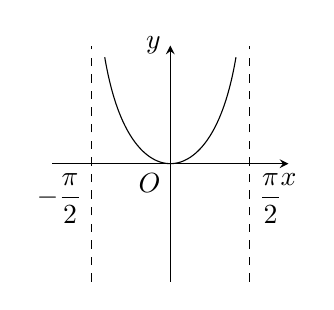
\begin{tikzpicture}[samples=200,>=stealth]
	\draw [->](-1.5,0)--(0,0) node [below left] {$O$}--(1.5,0) node [below] {$x$};
	\draw [->](0,-1.5)--(0,1.5) node [left] {$y$};
	\draw [dashed] (-1,-1.5)--(-1,1.5) (1,-1.5)--(1,1.5);
	\draw (-1,0) node [below left] {$-\dfrac{\pi}{2}$};
	\draw (1,0) node  [below right] {$\dfrac{\pi}{2}$};
	\draw [domain=-75:75] plot ({\x/90},{-ln(cos(\x))});
	\end{tikzpicture}}





\item 在实数集$\mathbf{R}$上定义运算$\otimes: x\otimes y=2x^2+y^2+1-y$, 则满足$x\otimes y=y\otimes x$的实数对$(x,y)$在平面直角坐标系中对应点的轨迹为\blank{30}.
\fourch{双曲线}{一条直线}{两条直线}{以上都不对}
\item 如图, 该几何体由半圆柱体与直三棱柱构成, 半圆柱体底面直径$BC=4$, $AB=AC$, $\angle BAC=90^\circ$, $D$为半圆弧$B_1C_1$的中点, 若异面直线$BD$和$AB_1$所成的角的大小为$\arccos\dfrac 23$, 求:\\
(1) 该几何体的体积;\\
(2) 直线$AC$与平面$ACC_1A_1$所成的角的大小.
\begin{center}
	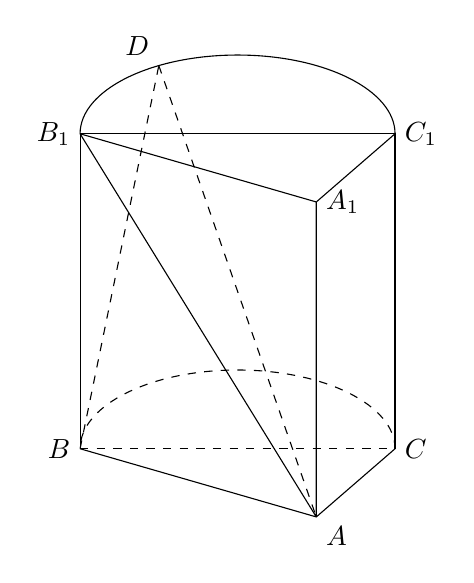
\begin{tikzpicture}
	\draw (-2,-2) node [left]{$B$} --(-2,2) node [left] {$B_1$} --(2,2) node [right]{$C_1$}--(2,-2) node [right] {$C$};
	\draw [dashed] (-2,-2)--(2,-2);
	\draw (2,2) arc (0:180:2 and 1);
	\draw [dashed] (2,-2) arc (0:180: 2 and 1);
	\path (2,2) arc (0:120:2 and 1) coordinate (D);
	\coordinate (A) at ($(0,0)!-1!(D)$);
	\coordinate (A1) at ($(0,2)!-1!(D)$);
	\draw [dashed] (D) node [above left] {$D$}--(A) node [below right]{$A$} (-2,-2)--(D);
	\draw (-2,-2)--(A)--(2,-2) (A)--(A1) node [right] {$A_1$} (-2,2)--(A1)--(2,2) (A)--(-2,2);
	\end{tikzpicture}
\end{center}
\item 设数列$\{a_n\}$的前$n$项和为$S_n$, 对任意的正整数$n$, 都有$a_n=5S_n+1$成立, 记$b_n=\dfrac{4+a_n}{1-a_n} \ (n\in\mathbf{N}^*)$.\\
(1) 求数列$\{b_n\}$的通项公式;\\
(2) 记$c_n=b_{2n}-b_{2n-1} \ (n\in \mathbf{N}^*)$, 设数列$\{c_n\}$的前$n$项和为$T_n$, 求证: 对任意正整数$n$都有$T_n<\dfrac 32$.
\item 已知集合$A=\{x|x=a+(a^2-1)\mathrm{i}\}$($a\in \mathbf{R}$, $\mathrm{i}$是虚数单位), 若$A\subseteq \mathbf{R}$, 则$a=$\blank{50}.
\item 在正方体$ABCD-A_1B_1C_1D_1$中, $M$和$N$分别为$A_1B_1$和$BB_1$的中点, 那么直线$AM$与$CN$所成角的余弦值是\blank{50}.
\item 计算$1-3\mathrm{C}_{10}^1+9\mathrm{C}_{10}^2-27\mathrm{C}_{10}^3+\cdots-3^9\mathrm{C}_{10}^9+3^{10}=$\blank{50}.
\item 在$\triangle ABC$中, 角$A,B,C$所对的边分别为$a,b,c$. 若$a=\sqrt{2}$, $b=2$, $\sin B+\cos B=\sqrt{2}$, 则角$A$的大小为\blank{50}.
\item (理科)已知两曲线参数方程分别为$\begin{cases}x=\sqrt{5}\cos\theta,\\y=\sin\theta,\end{cases} (0\le \theta<\pi)$和$\begin{cases}
x=\dfrac 54 t^2, \\ y=t, \end{cases}
(t\in \mathbf{R})$, 它们的焦点坐标为\blank{50}.
\item 从抛物线$y^2=4x$上一点$P$引抛物线的垂线, 垂足为$M$, 且$|PM|=5$, 设抛物线的焦点为$F$, 则$\triangle MPF$的面积为\blank{50}.
\item 在$\triangle ABC$中, 点$O$是$BC$的中点, 过点$O$的直线分别交直线$AB,AC$于不同的两点$M,N$, 若$\overrightarrow{AB}=m\overrightarrow{AM}, \overrightarrow{AC}=n\overrightarrow{AN}$, $m>0$, $n>0$, 则$\dfrac 1m+\dfrac 4n$的最小值为\blank{50}.
\item 已知$3$名志愿者在$10$月$1$日至$10$月$5$日期间参加$2013$年国庆节志愿者活动工作.\\
(文科)若每名志愿者在$5$天中任选一天参加社区服务工作, 且各志愿者的选择互不影响, 则$3$名志愿者恰好连续$3$天参加社区服务工作的概率为\blank{50}.\\
(理科)若每名志愿者在这$5$天中任选两天参加社区服务工作, 且各志愿者的选择互不影响, 以$\xi$表示这$3$名志愿者在$10$月$1$日参加志愿者服务工作的人数, 则随机变量$\xi$的数学期望为\blank{50}.
\item 已知对于任意非零实数$m$, 不等式$|5m-3|+|3-4m|\ge |m|\left(x-\dfrac 2x\right)$恒成立, 则实数$x$的取值范围是\blank{50}.
\item 已知圆的半径为$1$, $PA,PB$为该圆的两条切线, $A,B$为切点, 那么$\overrightarrow{PA}\cdot\overrightarrow{PB}$的最小值为\blank{50}.
\item 若$m,n$为两条不同的直线, $\alpha,\beta$为两个不同的平面, 则以下命题正确的是\blank{30}.
\twoch{若$m\parallel \alpha$, $n\parallel\alpha$, 则$m\parallel n$}{若$m\parallel \beta$, $\alpha\parallel\beta$, 则$m\parallel\alpha$}{若$m\parallel n$, $m\perp \alpha$, 则$n\perp \alpha$}{若$\alpha\cap\beta=m$, $m\perp n$, 则$n\perp\alpha$}
\item 双曲线$\dfrac{x^2}{a^2}-\dfrac{y^2}{b^2}=1$的左焦点为$F_1$, 顶点为$A_1,A_2$, $P$是该双曲线右支上任意一点, 则分别以线段$PF_1,A_1A_2$为直径的两圆一定\blank{30}.
\fourch{相交}{内切}{外切}{相离}
\item 方程$x^2+\sqrt{2}x-1=0$的解可视为函数$y=x+\sqrt{2}$的图像与函数$y=\dfrac 1x$的图像交点的横坐标, 若$x^4+ax-4=0$的各个实根$x_1,x_2,\cdots,x_k \ (k\le 4)$所对应的点$\left(x_i,\dfrac{4}{x_i}\right) \ (i=1,2,\cdots,k)$均在直线$y=x$的同侧, 则实数$a$的取值范围是\blank{30}.

\fourch{$(-\infty,-6)$}{$(6,+\infty)$}{$[-6,6]$}{$(-\infty,-6)\cup (6,+\infty)$}
\item 已知集合$M$是满足下列性质的函数$f(x)$的全体, 存在非零常数$T$, 对任意$x\in \mathbf{R}$, 有$f(x+T)=Tf(x)$成立.\\
(1) 函数$f(x)=x$是否属于集合$M$? 说明理由;\\
(2) 设$f(x)\in M$, 且$T=2$, 已知当$1<x<2$时, $f(x)=x+\ln x$, 求当$-3<x<-2$时, $f(x)$的解析式.
\item 在数列$\{a_n\}$中, 对于任意$n\in \mathbf{N}^*$, 等式$a_1+2a_2+2^2a_3+\dots+2^{n-1}a_n=(n\cdot 2^n-2^n+1)b$成立, 其中常数$b\ne 0$.\\
(1) 求$a_1,a_2$的值;\\
(2) 求证: 数列$\{2^{a_n}\}$为等比数列;\\
(3) 关于$n$的不等式$\dfrac{1}{a_2}+\dfrac{1}{a_4}+\dfrac{1}{a_8}+\cdots+\dfrac{1}{a_{2^n}}>\dfrac{c}{a_1} \ (c\in \mathbf{R})$的解集为$\{n|n\ge 3, \ n\in \mathbf{N}^*\}$, 求$b$和$c$应满足的条件.
\item 复数$\dfrac{(1+\mathrm{i})^2}{1-\sqrt{3}\mathrm{i}}$的模是\blank{50}.
\item 若$\begin{vmatrix}a_1 & b_1 & c_1\\1 & 2 & 3\\4 & 5 & 6\end{vmatrix}=a_1A_1+b_1B_1+c_1C_1$, 则$B_1$化简后的最后结果等于\blank{50}.
\item 已知集合$P=\{a,-1\}$, $Q=\{x|x^2-1<0, \ x\in \mathbf{Z}\}$, 如果$P\cap Q\ne\varnothing$, 则实数$a=$\blank{50}.
\item 若圆锥的侧面展开图是弧长为$2\pi$cm, 半径为$\sqrt{2}$cm的扇形, 则该圆锥的体积为\blank{50}cm$^3$.
\item 已知角$\alpha$的终边上一点的坐标为$\left(\sin\dfrac{2\pi}{3},\cos\dfrac{2\pi}{3}\right)$, 则角$\alpha$的最小正值为\blank{50}.
\item (理科)已知随机变量$\xi$的分布列如下表, 则随机变量$10\xi+1$的均值是\blank{50}.
\begin{center}
\begin{tabular}{|c|c|c|c|c|c|}
\hline
$x$ & $1$ & $2$ & $3$ & $4$ & $5$\\ \hline
$P(\xi=x)$ & $0.1$ & $a$ & $0.4$ & $0.1$ & $0.2$\\ \hline
\end{tabular}
\end{center}

\item 若函数$f(x)=2\cos\left(\dfrac{\pi}{3}x-\dfrac{\pi}{6}\right) \ (-1<x<5)$的图像与$x$轴交于点$A$, 过点$A$的直线$l$与函数的图像交于另外两点$B,C$. $O$是坐标原点, 则$(\overrightarrow{OB}+\overrightarrow{OC})\cdot\overrightarrow{OA}=$\blank{50}.
\item 设$(1+x)+(1+x)^2+\cdots+(1+x)^n=a_0+a_1x+a_2x^2+\cdots+a_nx^n, \ n\in \mathbf{N}^*$, 若$a_1+a_2+\cdots+a_{n-1}=61-n$, 则$n=$\blank{50}.
\item 若存在$x\in [0,1]$, 使不等式$x^2+x\ge a^2+a$成立, 则实数$a$的取值范围是\blank{50}.
\item $F$为双曲线$C: \dfrac{x^2}{64}-\dfrac{y^2}{16}=1$的左焦点, 双曲线$C$上的点$P_i$与$P_{7-i} \ (i=1,2,3)$关于$y$轴对称, 且$P_1,P_2,P_3$在双曲线的右支上, 则$|P_1F|+|P_2F|+|P_3F|-|P_4F|-|P_5F|-|P_6F|$的值是\blank{50}.
\item (文科)已知非零实数$a,b$满足$a>b$. 则下列不等式中成立的是\blank{30}.
\fourch{$a^2>b^2$}{$\dfrac 1a<\dfrac 1b$}{$a^2b>ab^2$}{$\dfrac{a}{b^2}>\dfrac{b}{a^2}$}\\
(理科)对任意的实数$\alpha,\beta$, 下列等式恒成立的是\blank{30}.
\twoch{$2\sin\alpha\cdot\cos\beta=\sin(\alpha+\beta)+\sin(\alpha-\beta)$}{$2\cos\alpha\cdot\sin\beta=\sin(\alpha+\beta)+\cos(\alpha-\beta)$}{$\cos\alpha+\cos\beta=2\sin\dfrac{\alpha+\beta}{2}\cdot\sin\dfrac{\alpha-\beta}{2}$}{$\cos\alpha-\cos\beta=2\cos\dfrac{\alpha+\beta}{2}\cdot\cos\dfrac{\alpha-\beta}{2}$}
\item (理科)已知函数$f(x)$是定义在$\mathbf{R}$上的单调递减函数且为奇函数, 数列$\{a_n\}$是等差数列, $a_{1007}>0$, 则$f(a_1)+f(a_2)+f(a_3)+\cdots+f(a_{2012})+f(a_{2013})$的值\blank{30}.
\fourch{恒为正数}{恒为负数}{恒为$0$}{可正可负}
\item 已知$A,B$为平面内两定点, 过该平面内动点$M$作直线$AB$的垂线, 垂足为$N$. 若$\overrightarrow{MN}^2=\lambda \overrightarrow{AN}\cdot\overrightarrow{NB}$, 其中$\lambda$为常数, 则动点$M$的轨迹不可能是\blank{50}.
\fourch{圆}{椭圆}{抛物线}{双曲线}
\item (文科)如图, 在正三棱柱$ABC-A_1B_1C_1$中, $AA_1=6$, 异面直线$BC_1$与$AA_1$所成角的大小为$\dfrac{\pi}{6}$, 求该三棱柱的体积和表面积.\\
(理科)在等腰直角三角形$ABC$中, $\angle A=90^\circ$, $BC=6$, $D,E$分别是$AC,AB$上的点, $CD=BE=\sqrt{2}$, $O$为$BC$的中点. 将$\angle ADE$沿$DE$折起, 得到如图所示的四棱锥$A'-BCDE$, 其中$A'O=\sqrt{3}$.\\
(1) 证明: $A'O\perp$平面$BCDE$;\\
(2) 求二面角$A'-CD-B$的平面角的余弦值.
\begin{center}
	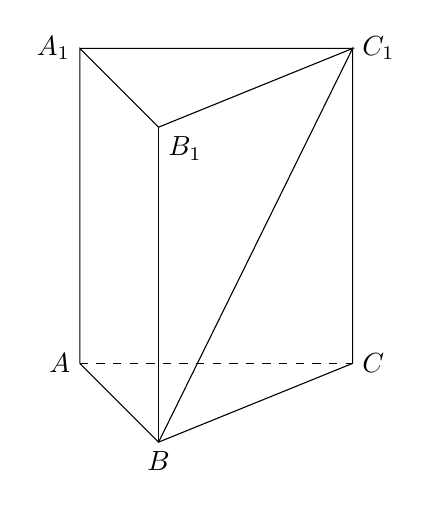
\begin{tikzpicture}
	\draw [dashed](0,0) node [left] {$A$}--({2*sqrt(3)},0) node [right] {$C$};
	\path (1,-1) coordinate (B);
	\path (1,3) coordinate (B1);
	\draw (0,0)--(B)--({2*sqrt(3)},0);
	\draw (B) node [below] {$B$}--(B1) node [below right] {$B_1$};
	\draw (0,0)--(0,4) node [left] {$A_1$}--(B1)--({2*sqrt(3)},4) node [right] {$C_1$}--(0,4) ({2*sqrt(3)},0)--({2*sqrt(3)},4)--(B);
	\end{tikzpicture}
	
	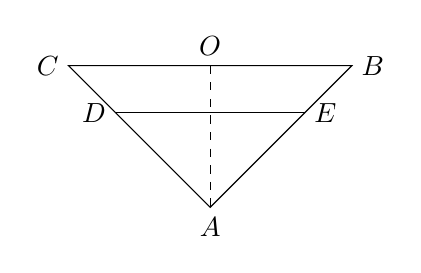
\begin{tikzpicture}
	\draw (-1.8,0) node [left] {$C$}--(0,0) node [above] {$O$}--(1.8,0) node [right] {$B$}--(0,-1.8) node [below] {$A$}--cycle;
	\draw (-1.2,-0.6) node[left] {$D$}--(1.2,-0.6) node  [right] {$E$};
	\draw [dashed] (0,0)--(0,-1.8);
	\end{tikzpicture}
	
	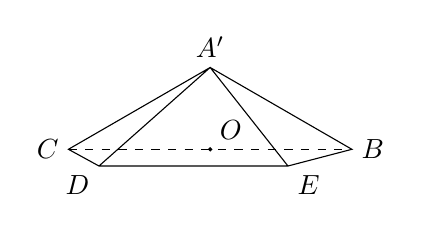
\begin{tikzpicture}
	\path (-1.8,0) coordinate (C) --(0,0) coordinate (O) --(1.8,0) coordinate (B);
	\path (0.9,0) arc (0:-135:0.9) coordinate (P);
	\coordinate (D) at ($(C)!{1/3}!(P)$);
	\coordinate (E) at ($(B)!{1/3}!(P)$);
	\coordinate (A') at (0,{0.6*sqrt(3)});
	\draw (C) node [left] {$C$}--(D) node [below left] {$D$}--(E) node [below right] {$E$}--(B) node [right] {$B$}--(A') node [above] {$A'$} --cycle (D)--(A')--(E);
	\draw [dashed] (C)--(0,0)  node[above right] {$O$}--(B);
	\filldraw (0,0) circle (0.02);
	\end{tikzpicture}
\end{center}
\item 如图, 某市拟在长为$8$千米的道路$OP$的一侧修建一条运动赛道, 赛道的前一部分为曲线段$OSM$, 该曲线段为函数$y=A\sin \omega x \ (A>0,\omega>0), \ x\in [0,4]$的图像, 且图像的最高点为$S(3,2\sqrt{3})$; 赛道的后一部分为折线段$MNP$, 为保证参赛运动员的安全, 限定$\angle MNP=\dfrac{2\pi}{3}$.\\
(1) 求$A,\omega$的值和线段$MP$的长;\\
(2) 设$\angle PMN=\theta$, 问$\theta$为何值时, 才能使折线段赛道$MNP$最长?
\begin{center}
	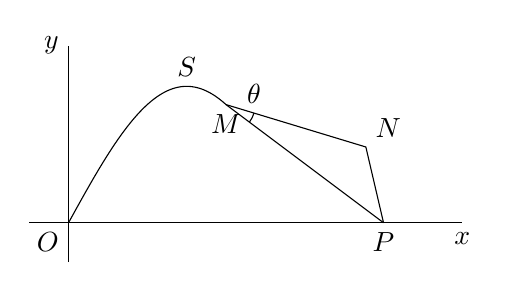
\begin{tikzpicture}[scale=0.5,samples=200,>=stealth]
	\draw (-1,0)--(0,0) node [below left] {$O$}--(10,0) node [below] {$x$};
	\draw (0,-1)--(0,4.5) node [left] {$y$};
	\draw [domain=0:4] plot (\x,{2*sqrt(3)*sin(\x*30)});
	\draw (3,{2*sqrt(3)}) node [above]{$S$};
	\draw (4,3) node [below] {$M$};
	\draw (4,3)--(8,0) node [below] {$P$};
	\coordinate (D) at ($(4,3)!{2/sqrt(3)*sin(40)}!(8,0)$);
	\path (D) arc ({-atan(3/4)}:{-atan(3/4)+20}:{10/sqrt(3)*sin(40)}) coordinate (N);
	\draw (4,3)--(N) node [above right] {$N$}--(8,0);
	\draw ($(4,3)!{0.4/sqrt(3)*sin(40)}!(8,0)$)   arc ({-atan(3/4)}:{-atan(3/4)+20}:{2/sqrt(3)*sin(40)}) node[above]{$\theta$};
	\end{tikzpicture}
\end{center}
\item 已知平面$\alpha\cap$平面$\beta=l$, 直线$a\subsetneqq\alpha$, 直线$b\subsetneqq \beta$, 则``$a$与$b$是异面直线''是``$a,b$均与$l$相交且交点不同''的\blank{50}条件.
\item 函数$y=\arcsin(1-x)+\arccos x$的值域是\blank{50}.
\item (理科)在极坐标系中, 方程$\rho=3\cos^2\dfrac{\theta}{2}-\sin^2\dfrac{\theta}{2}-1$表示的曲线是\blank{50}.\\
(文科)某学校要把$9$台型号相同的电脑送给某地区的三所小学, 每所小学至少得到$2$台, 则不同的送法有\blank{50}种.
\item (理科)极坐标中的曲线$\rho=2$与$\rho\sin\theta=m$有两个公共点, 则$m$的取值范围是\blank{50}.\\
(文科)已知$a,b$为不垂直的异面直线, $\alpha$是一个平面, 则$a,b$在$\alpha$上的射影有可能是

\textcircled{1} 两条平行直线; \textcircled{2} 两条互相垂直的直线; \textcircled{3} 同一条直线; \textcircled{4} 一条直线及其外一点.

上面的结论中, 正确结论的编号是\blank{50}.
\item (理科)在正三棱柱$ABC-A_1B_1C_1$中, 各棱长均为$4$, $M,N$分别是棱$BC,CC_1$的中点, 则二面角$B-AM-B_1$的正切值为\blank{50}, 三棱锥$B-AB_1-N$的体积为\blank{50}.
\item 在$\triangle ABC$中, $\angle C=90^\circ$, 则$\cos A\cos B$的取值范围是\blank{50}.
\item 设$\left(3x^{\frac 13}+x^\frac 12\right)^n$展开式的各项系数之和为$t$, 其二项式系数之和为$h$, 且$t+h=272$, 则展开式中$x^2$的系数为\blank{50}.
\item 甲、乙、丙三个单位分别需要招聘工作人员$2$名、$1$名、$1$名, 现从$10$名应聘人员中招聘$4$人到甲、乙、丙三个单位, 那么不同的招聘方法共有\blank{50}种.
\item (理科)曲线$\rho=-2\sin\theta$与$\theta=\dfrac{\pi}{6} \ (\rho>0)$的交点个数是\blank{50}.\\
(文科)从一副扑克牌($52$张)中任取$4$张, $4$张花色各不相同的概率是\blank{50}.
\item 某商场开展促销抽奖活动, 摇奖器摇出一组中奖号码为$1,2,3,4,5,6$, 参加抽奖的顾客从$0$至$9$十个号码中任意抽取$6$个, 若其中至少有$5$个号码与摇奖器摇出的号码相同(不计顺序), 则可中奖. 那么某顾客抽一次就能中奖的概率为\blank{50}.
\item (理科)在极坐标系中, ``点$P$是极点''是``点$P$的极坐标是$(0,0)$''成立的\blank{30}.
\fourch{充分不必要条件}{必要不充分条件}{充要条件}{既不充分也不必要条件}\\
(文科)$\overrightarrow a,\overrightarrow b$为非零向量, ``函数$f(x)=(x\overrightarrow a+\overrightarrow b)^2$为偶函数''是``$\overrightarrow a\perp \overrightarrow b$''的\blank{30}.
\fourch{充分不必要条件}{必要不充分条件}{充要条件}{既不充分也不必要条件}
\item (理科)在方程为$\begin{cases}
x=\sin 2\theta,\\ y=\sin\theta+\cos\theta
\end{cases}$的曲线上的点是\blank{30}.
\fourch{$(2,\sqrt{3})$}{$(1,\sqrt{3})$}{$\left(-\dfrac 34,\dfrac 12\right)$}{$\left(\dfrac 12,-\sqrt{2}\right)$}\\
(文科)若函数$y=f(x)$存在反函数, 则方程$f(x)=c$($c$为常数)\blank{30}.
\fourch{有且只有一个实根}{至少有一个实根}{至多有一个实根}{没有实数根}
\item 设$M$是球$O$半径$OP$的中点, 分别过$M,O$作垂直于$OP$的平面, 截球面得两个圆, 则这两个圆的面积比值为\blank{30}.
\fourch{$\dfrac 14$}{$\dfrac 12$}{$\dfrac 23$}{$\dfrac 34$}
\item (理科)(1) 甲同学从学校乘车回家, 图中有$3$个交通岗, 假设在各交通岗遇到红灯的时间是相互独立的, 并且概率都是$\dfrac 25$, 求甲同学回家途中遇到红灯次数的期望值;\\
(2) $A$箱内有$1$个红球和$n+1$个白球, $B$箱内有$n-1$个白球($n\in \mathbf{N}, \ n\ge 2$), 现随机从$A$箱内取出$3$个球放入$B$箱内, 将$B$箱中的球充分搅拌后, 再从中随机取出$3$个球放入$A$箱, 求红球由$A$箱入$B$箱再返回$A$箱的概率.
\item 把边长为$a$的正方形减去图中的阴影部分, 沿图中所画折线折成一个正三棱锥, 求这个正三棱锥的高.
\begin{center}
	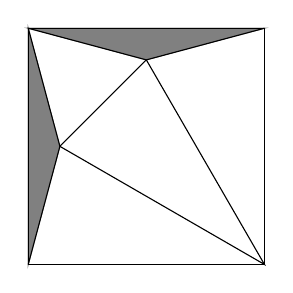
\begin{tikzpicture}
	\coordinate (P) at ({3/2},{3*sqrt(3)/2});
	\coordinate (Q) at ({3-3*sqrt(3)/2},{3/2});
	\filldraw [gray] (0,0)--(Q)--(0,3)--cycle;
	\filldraw [gray] (0,3)--(P)--(3,3)--cycle;
	\draw (0,0) rectangle (3,3);
	
	\draw (0,0)--(Q)--(P)--(3,3);
	\draw (0,3)--(Q)--(3,0)--(P)--cycle;
	\end{tikzpicture}
\end{center}
\item 在正方体$ABCD-A_1B_1C_1D_1$中, $E,F,G,H$分别为$AB_1,AB,BB_1,B_1C_1$的中点, 则异面直线$EF,GH$所成角的大小为\blank{50}.
\item 若一个球的体积为$4\sqrt{3}\pi$, 则它的表面积为\blank{50}.
\item 一个圆锥的侧面积是其底面积的$2$被, 则圆锥的母线与点所成的角为\blank{50}.
\item 已知正三棱锥的侧棱长是底面边长的$2$倍, 则侧棱与底面所成角的余弦值等于\blank{50}.
\item 正三棱锥$P-ABC$的高为$2$, 侧棱与底面$ABC$成$45^\circ$角, 则点$A$到侧面$PBC$的距离为\blank{50}.
\item (文科)一个扇形的半径为$30$cm, 圆心角为$120^\circ$, 用它做成一个圆锥的侧面, 那么这个圆锥的底面半径为\blank{50}.\\
(理科)函数$y=\sin\left(x+\dfrac{\pi}{12}\right)+\sin\left(x+\dfrac{5\pi}{12}\right), \ x\in [0,\pi]$的最大值为\blank{50}.
\item 若$(x-2)^5=a_5x^5+a_4x^4+a_3x^3+a_2x^2+a_1x+a_0$, 则$a_1+a_2+a_3+a_4+a_5=$\blank{50}.
\item 甲、乙、丙$3$位同学选修课程, 从$4$门学科中, 甲选$2$门, 乙、丙各选$3$门, 则不同的选修方案为\blank{50}.
\item 在正方体上任意选择两条棱, 则这两条棱平行的概率是\blank{50}.
\item (理科)已知极坐标系中, 圆心的极坐标为$\left(1,\dfrac{\pi}{3}\right)$, 半径为$1$, 则该圆的极坐标方程是\blank{50}.
\item 对于两条不相交的空间直线$a$和$b$, 一定存在平面$\alpha$, 使得\blank{30}.
\twoch{直线$a,b$均在平面$\alpha$内}{直线$a$在平面$\alpha$内, $b$与平面$\alpha$平行}{直线$a,b$都垂直于平面$\alpha$}{直线$a$在平面$\alpha$内, $b$与平面$\alpha$垂直}
\item 过球面上两点作球的大圆, 可能的个数是\blank{30}.
\fourch{有且只有一个}{一个或无穷多个}{无数个}{以上结论都不正确}
\item 如果$\left(3x^2-\dfrac{2}{x^3}\right)^n$的展开式中含有非零常数项, 那么正整数$n$的最小值为\blank{30}.
\fourch{$10$}{$6$}{$5$}{$3$}
\item 甲、乙等$5$位奥运志愿者被分到$A,B,C,D$四个不同的岗位上, 每个岗位至少有一名志愿者, 不同的分配方案概率相灯.\\
(1) 求甲乙两人同时参加$A$岗位服务的概率;\\
(2) (文科)求甲乙两人不在同一岗位服务的概率;\\
(理科)设随机变量$\xi$表示这$5$名志愿者中参加$A$岗位服务的人数, 求随机变量$\xi$的概率分布律.
\item 如图, 在Rt$\triangle ABC$中, $\angle C=90^\circ$, $BC=3$, $AC=6$, $D,E$分别是$AC,AB$上的点, 且$DE\parallel BC$, $DE=2$. 将$\triangle ADE$沿$DE$折起到$\angle A_1DE$的位置, 使$A_1C\perp CD$, 如图, $M$是$A_1D$的中点.\\
(1) 求证: $A_1C\perp$平面$BCDE$;\\
(2) (文科)求$CM$与平面$A_1DE$所成角的大小;\\
(理科)求$CM$与平面$A_1BE$所成角的大小.
\begin{center}
	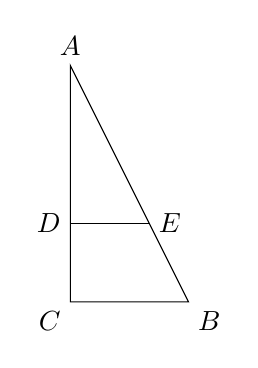
\begin{tikzpicture}
	\draw (0,0) node [below left] {$C$}--(1.5,0) node [below right] {$B$}--(0,3) node [above] {$A$}--cycle;
	\draw (0,1) node [left] {$D$}--(1,1) node [right] {$E$};
	\end{tikzpicture}
	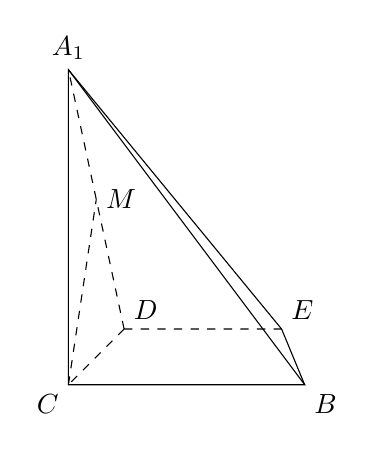
\begin{tikzpicture}
	\draw (0,0) node [below left] {$C$} --(3,0) node [below right] {$B$}-- (0,4) node [above] {$A_1$} --cycle;
	\coordinate (D) at ({sqrt(2)/2},{sqrt(2)/2});
	\path (D)--+(2,0) coordinate (E);
	\draw (3,0)--(E) node [above right] {$E$}--(0,4);
	\draw [dashed] (D) node [above right] {$D$}--(E) (D)--(0,0) (D)--(0,4); 
	\coordinate (M) at ($(0,4)!0.5!(D)$);
	\draw [dashed] (0,0)--(M) node [right] {$M$};
	\end{tikzpicture}
\end{center}

\end{enumerate}
\end{document}